\documentclass[12pt,a4paper,twoside]{report}

%Paczki ----------------------------------------------------------------
\usepackage{polski}					%Język dokumentu
\usepackage[utf8]{inputenc}			%Kodowanie znaków
\usepackage[table]{xcolor}			%Kolory w tabeli
\usepackage{hyperref}				%Hiperłącza
\usepackage{amsmath}
\usepackage{amsfonts}
\usepackage{amssymb}
\usepackage{multirow}				%Macierze z dużą ilością wierszy
\usepackage{mathtools}
\usepackage{pdfpages}				%Wstawienie pdf ze stroną tytułową
\usepackage{appendix}				%Rozdział z dodatkami
\usepackage{color}					%Kolorowanie tekstu
\usepackage{float}					%Pozycjonowanie rysunków
\usepackage{epstopdf}				%Konwesja eps do pdf
\usepackage{fancyhdr}
\usepackage{rotating}				%Obracanie tabeli
\usepackage{listings}				%Kod źródłowy
\usepackage{nomencl}				%Spis oznaczeń użytych w projekcie
\usepackage{graphicx}				%Wstawianie rysunków
\usepackage{caption}
\usepackage{subcaption}				%Podpisy pod wieloobrazkami




%Rozmiar macierzy------------------------------------------------------
\setcounter{MaxMatrixCols}{20} 



%Żywa pagina-----------------------------------------------------------
\pagestyle{fancy}
\renewcommand{\chaptermark}[1]{\markboth{#1}{}}
\renewcommand{\sectionmark}[1]{\markright{\thesection\ #1}}
\fancyhf{} % usun biezace ustawienia pagin
\fancyhead[LE,RO]{\small\bfseries\thepage}
\fancyhead[LO]{\small\bfseries\rightmark}
\fancyhead[RE]{\small\bfseries\leftmark}
\renewcommand{\headrulewidth}{0.5pt}
\renewcommand{\footrulewidth}{0pt}
\addtolength{\headheight}{0.5pt} % pionowy odstep na kreske
\fancypagestyle{plain}{	%Strony z początkiem rozdziału
	\fancyhead{} 		% usun p. górne na stronach pozbawionych numeracj
	\renewcommand{\headrulewidth}{0pt}	%Zerowa grubość poziomej kreski
}



%Przesunięcie tytułu rozdziału w górę strony-----------------------------
\usepackage{titlesec}
\titlespacing*{\chapter}{0pt}{-20pt}{20pt}
\titleformat{\chapter}[display]{\normalfont\huge\bfseries}{\chaptertitlename\ \thechapter}{20pt}{\Huge}



%Marginesy---------------------------------------------------------------
\evensidemargin = 10pt	%=10pt
\oddsidemargin 	= 40pt 	%=50pt


%Cytowanie w stopce strony-----------------------------------------------
\usepackage[style=verbose,autocite=footnote,maxnames=10,babel=hyphen,hyperref=true,abbreviate=false,backend=biber]{biblatex} 



%Kod źródłowy-------------------------------------------------------------
\usepackage{caption}
\DeclareCaptionFont{white}{\color{white}}
\DeclareCaptionFormat{listing}{\colorbox{gray}{\parbox{\textwidth}{#1 #2#3}}}
\captionsetup[lstlisting]{format=listing,labelfont={bf,white},textfont=white}
\renewcommand\lstlistingname{Kod źródłowy}												

%Formatowanie kodu źródłowego C++ --------------------
\definecolor{dark_green}{rgb}{0,0.6,0}		%Definicja koloru zielonego
\definecolor{light-gray}{gray}{0.93}		%Definicja koloru jasnoszarego
\lstdefinestyle{nonumbers}{numbers=none}	%Brak numeracji listeningu
\lstset{
	language		= C++,					%Język programowania
	commentstyle	= \color{dark_green},	%Kolor komentarzy
	extendedchars	= false,
	escapeinside	= '',
	numbers			= left,					%Numerowanie linii kodu
	numbersep		= 2pt,					%Odsunięcie numeracji od kodu 
	numberstyle		= \color{blue},			%Kolor numerów linii kodu
	stepnumber		= 2, 					%Widoczne numery linii kodu
	basicstyle		= \footnotesize,		%Format tekstu
	tabsize			= 4,					%Wielkość wcięć
	backgroundcolor = \color{light-gray},	%Kolor tła
	morekeywords	= {cPoint,std,string,eSolutionType,POISSON,
						DISTANCE,cout,endl,cSolver,TECPLOT}	%Pogrubienie dodatkowych słów kluczowych
}



%Dodanie nawiasów klamrowych do \ref -----------------------------
\let\oldtheequation\theequation
\makeatletter
\def\tagform@#1{\maketag@@@{\ignorespaces#1\unskip\@@italiccorr}}
\renewcommand{\theequation}{(\oldtheequation)}
\renewcommand{\theequation}{(\oldtheequation)}
\makeatother 



%Wyczyszczenie z nagłówka pustej strony (nadpisanie \cleardoublepage)
\let\origdoublepage\cleardoublepage
\newcommand{\clearemptydoublepage}{%
  \clearpage
  {\pagestyle{empty}\origdoublepage}%
}



\author{Marcin Stelmaszyk}			
\title{Wyznaczenie odległości od brzegu w oparciu o równania różniczkowe cząstkowe.}



%Struktura dokumentacji--------------------------------------------------
\begin{document}
	%Strony początkowe
	
\includepdf{strona_tytulowa.pdf}	%Strona tytułowa
	
	\clearemptydoublepage 				%Spis treści od strony nieparzystej 
	\tableofcontents					%Spis treści
	\clearemptydoublepage 				%Wprowadzenie od strony nieparzystej
	\chapter{Wprowadzenie}
\section{Opis projektu}

\indent\indent Odległość od brzegu, $d$, pozostaje nadal kluczowym parametrem przy modelowaniu turbulencji oraz generowaniu siatek obliczeniowych\footcite{Tucker}.

\indent Celem niniejszego projektu jest opracowanie programu  umożliwiającego wyznaczanie minimalnej odległości między danym węzłem siatki, a brzegiem profilu lotniczego.
 
Najprostszym sposobem rozwiązania powyższego zagadnienia jest  bezpośrednie obliczenie odległości $d$ danego węzła $P$ od kolejnych węzłów $S$ należących do brzegu profilu korzystając z miary euklidesowej:

\begin{equation}
d(P,S)= \sqrt{(x_p-x_s)^2 + (y_p-y_s)^2}
\end{equation}

\noindent a następnie wybranie najmniejszej wartości z utworzonego zbioru odległości $\{d_0, d_1, ..., d_n\}$. Metoda ta, znana w terminologii algorytmicznej jako \textit{metoda siłowa} (ang. \textit{Brute Force}), jest łatwa do zaimplementowania, a liczba operacji potrzebnych do jej wykonania dla siatek stałych w czasie jest mała w stosunku do kosztu całego rozwiązania. Niemniej jednak, szybkie znalezienie odległości od brzegu ma kluczowe znaczenie dla problemów rozwiązywanych przy użyciu siatek deformujących się i adaptacyjnych, dla których wyznaczenie minimalnej odległości od brzegu jest przeprowadzane wielokrotnie\footcite{Ibid}. 

Innym podejściem jest wykorzystanie równań różniczkowych cząstkowych. Do rozwiązania problemu Sethain\footcite{Sethain} zaproponował wykorzystanie równania Eikonału następującej postaci

\begin{equation}
\label{eq:eikonal}
\left|\nabla \phi\right|=1+\lambda\nabla^2\phi
\end{equation}

\newpage
\indent Niniejszy projekt skupi się na implementacji uproszczonej  jego wersji, a mianowicie równaniu Poissona na płaszczyźnie $(x,y)$

\begin{equation}
\nabla^2\phi = - 1
\end{equation}

\indent Pomocniczo została utworzona siatka obliczeniowa wokół profilu, o strukturze dopasowanej do zadanego brzegu obszaru. Tak zdefiniowana przestrzeń fizyczna została przetransformowana do przestrzeni obliczeniowej, a następnie zdyskretyzowana metodą różnic skończonych. Powstały układ równań algebraicznych rozwiązano metodą iteracyjną. Otrzymane wyniki skonfrontowano z rozwiązaniem siłowym.

\indent Program został zaimplementowany w języku C++ przy użyciu darmowego środowiska programistycznego Microsoft Visual Studio Express 2012\footnote{\url{www.microsoft.com/visualstudio/}}. Język C++ ma szerokie zastosowanie w programach obliczeniowych, więc jego wykorzystanie umożliwia integrację w istniejących lub przyszłych kodach obliczeniowych. Do wizualizacji wyników skorzystano z programu \textsf{Tecplot 360}\footnote{\url{www.tecplot.com}}.

\indent Niniejsza dokumentacja została stworzona w języku \LaTeX\quad przy użyciu edytora \textsf{TexMaker 3.5.2}\footnote{\url{http://www.xm1math.net/texmaker/}}.
	\chapter{Model matematyczny}

\section{Równanie Eikonału}

\indent\indent Zmienna $\phi$ w równaniu Eikonału \ref{eq:eikonal} modeluje czas przybycia frontu fali propagującej od powierzchni brzegu. Prawa strona równania wskazuje na jednostkową prędkość tego frontu, tzn. istnieje pole prędkości o $|\textbf{U}|=1$, co oznacza, że wyznaczona wartość jest równa szukanej odległości $d$\footcite{Tucker}.

\indent Zmodyfikowana forma równania z jawnym laplasjanem, jak poniżej, jest zwana równaniem Hamiltona-Jacobiego

\begin{equation}
\textbf{U}\circ\nabla\phi = 1 + \Gamma(\phi)\nabla^2\phi
\label{eq:eikonal_2}
\end{equation}

\indent Rozwiązanie \ref{eq:eikonal_2}, w oparciu o początkowy rozkład wartości $\phi$, otrzymuje się w sposób iteracyjny.
\section{Równanie Poissona}
\indent\indent Przy założeniu, że $\textbf{U}=0$ oraz $\Gamma = 1$, równanie \ref{eq:eikonal_2} można sprowadzić do równania Poissona 

\begin{equation}
\nabla^2 \phi = -1 \iff \frac{\partial^2 \phi}{\partial x^2} + \frac{\partial^2 \phi}{\partial y^2} = -1
\label{eq:poisson_1}
\end{equation}

\noindent Wstawiając wartości otrzymanego rozwiązania $\phi$ do zależności


\begin{equation}
d = - \sqrt{\left(\frac{\partial\phi}{\partial x}\right)^2+\left(\frac{\partial\phi}{\partial y}\right)^2}+\sqrt{\left(\frac{\partial\phi}{\partial x}\right)^2+\left(\frac{\partial\phi}{\partial y}\right)^2+2\phi}
\label{eq:d_1}
\end{equation}

\noindent otrzymuje się poszukiwaną odległość od brzegu. Należy mieć na uwadze, że wyprowadzenie wzoru \ref{eq:d_1} wymaga przyjęcia nieskończonych współrzędnych poza kierunkiem normalnym do brzegu. Oznacza to, że rozwiązanie jest dokładne tylko blisko ściany. Nie stanowi to znaczącego problemu w modelach turbulencji, bowiem korzystają one tylko z wartości $d$ wyznaczonych blisko brzegu\footnote{A ściślej - maksymalnie do jednej trzeciej grubości warstwy przyściennej (\textbf{ibid.})}

\section{Transformacja siatki z przestrzeni fizycznej do obliczeniowej}

\indent\indent W ramach niniejszego projektu została wygenerowana strukturalna siatka obliczeniowa o topologii typu O (ang. \textit{O-grid topology}), charakteryzująca się tym, że każdy z jej rzędów ($v=const$) tworzy wokół profilu krzywą zamkniętą, natomiast druga rodzina krzywych ($u=const$) rozciąga się prostoliniowo od powierzchni profilu (rys.~\ref{fig:siatka_krzywoliniowa}). Krzywa $v = 0$ pokrywa się z obwiednią profilu (od punktu \textsf{a} do \textsf{a'}), a linie $u=0$ (węzły \textsf{a}~-~\textsf{c}) oraz $u=u_{max}$ (węzły \textsf{a'}~-~\textsf{c'}) tną siatkę w przestrzeni obliczeniowej. Wadą topologii typu O jest słaba jakość siatki w miejscu ostrej krawędzi spływu, co wpływa na poprawność rozwiązania w tym obszarze\footcite{Blazek, s. 359}\footnote{Należy mieć na uwadze, że dobranie powyższego typu siatki, oraz sam fakt jej generowania w programie, jest czynnością pomocniczą wobec celu niniejszego projektu i służy jedynie sprawdzeniu poprawności implementacji modelu matematycznego.}.

\begin{figure}[H]
	\centering
	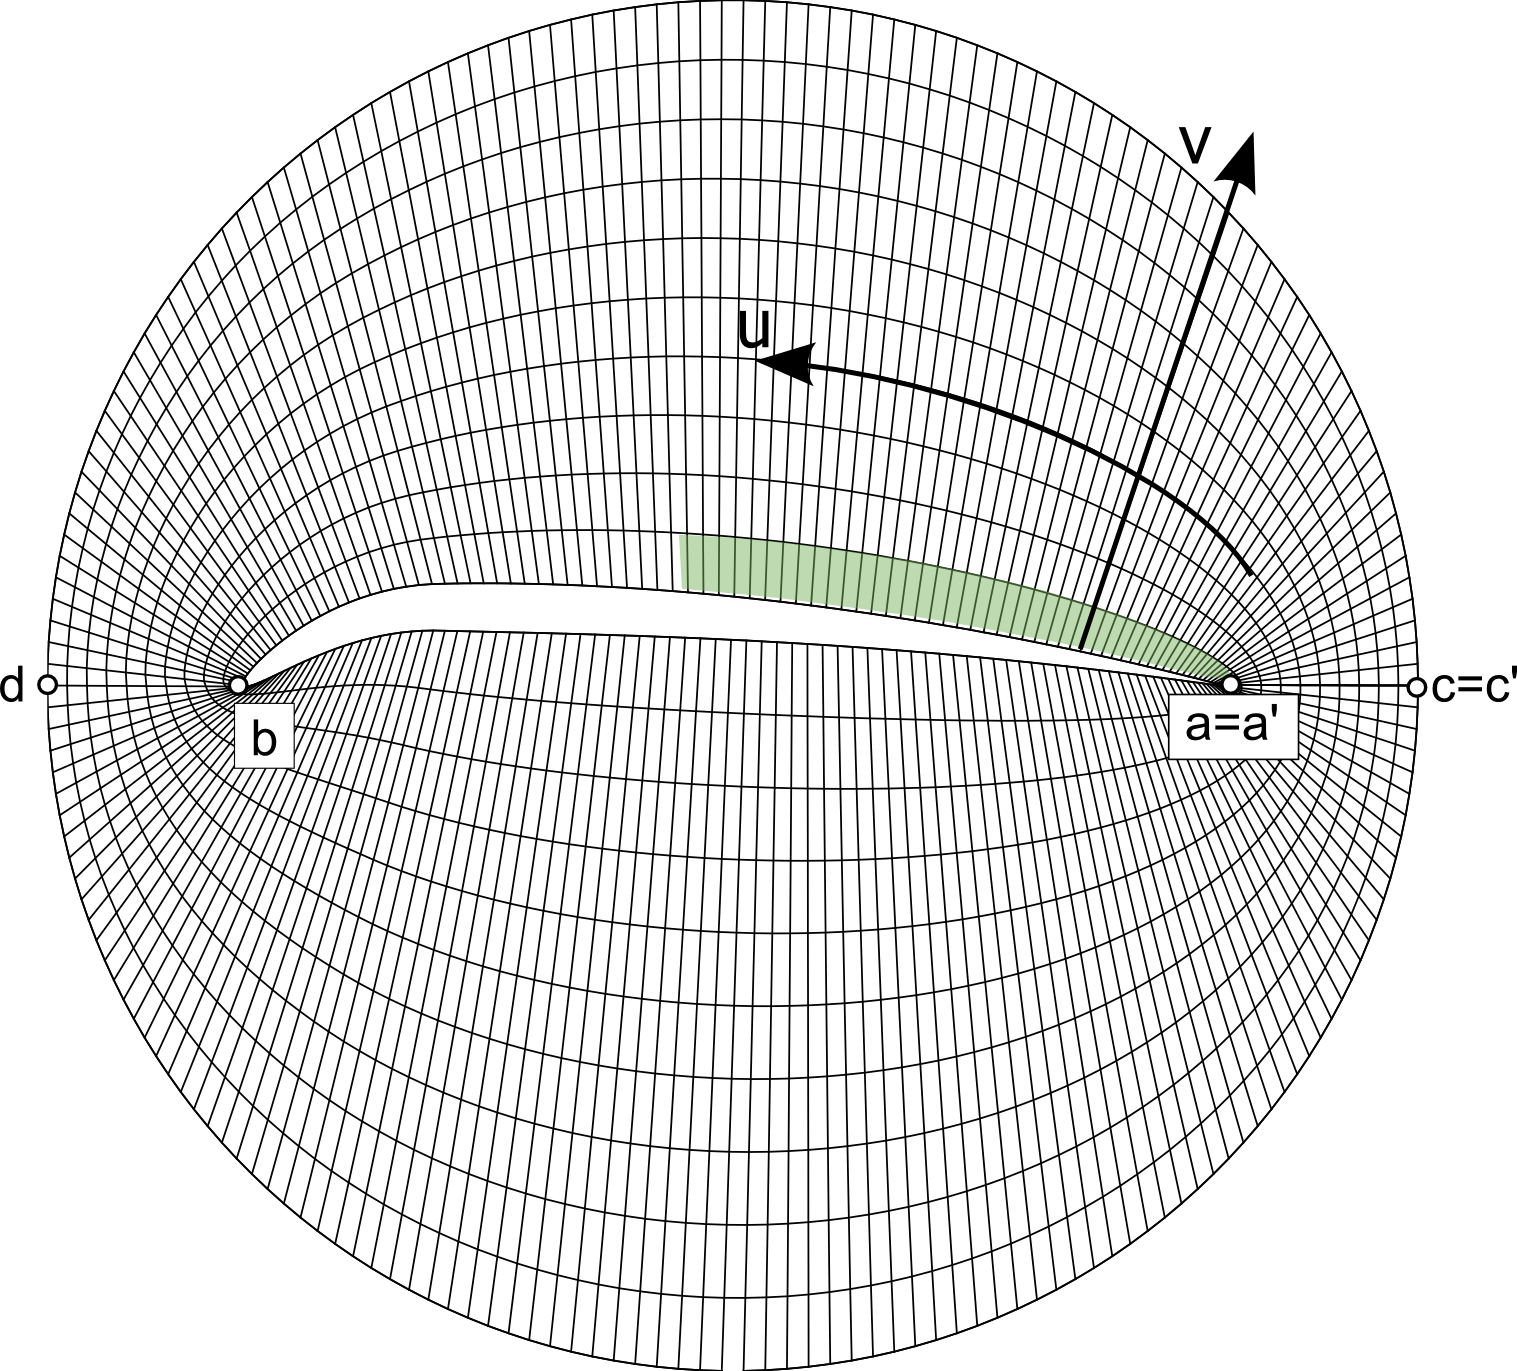
\includegraphics[width=0.8\linewidth]{Rysunki/siatka_krzywoliniowa.png}  
	\caption{Przestrzeń fizyczna. W oparciu o węzły leżące na konturze profilu została wygenerowana siatka krzywoliniowa o topologii O. Strzałkami oznaczono kierunki zmiennych $(u,v)$ z przestrzeni obliczeniowej. 
	\label{fig:siatka_krzywoliniowa}}
\end{figure} 

\begin{figure}[H]
	\centering
	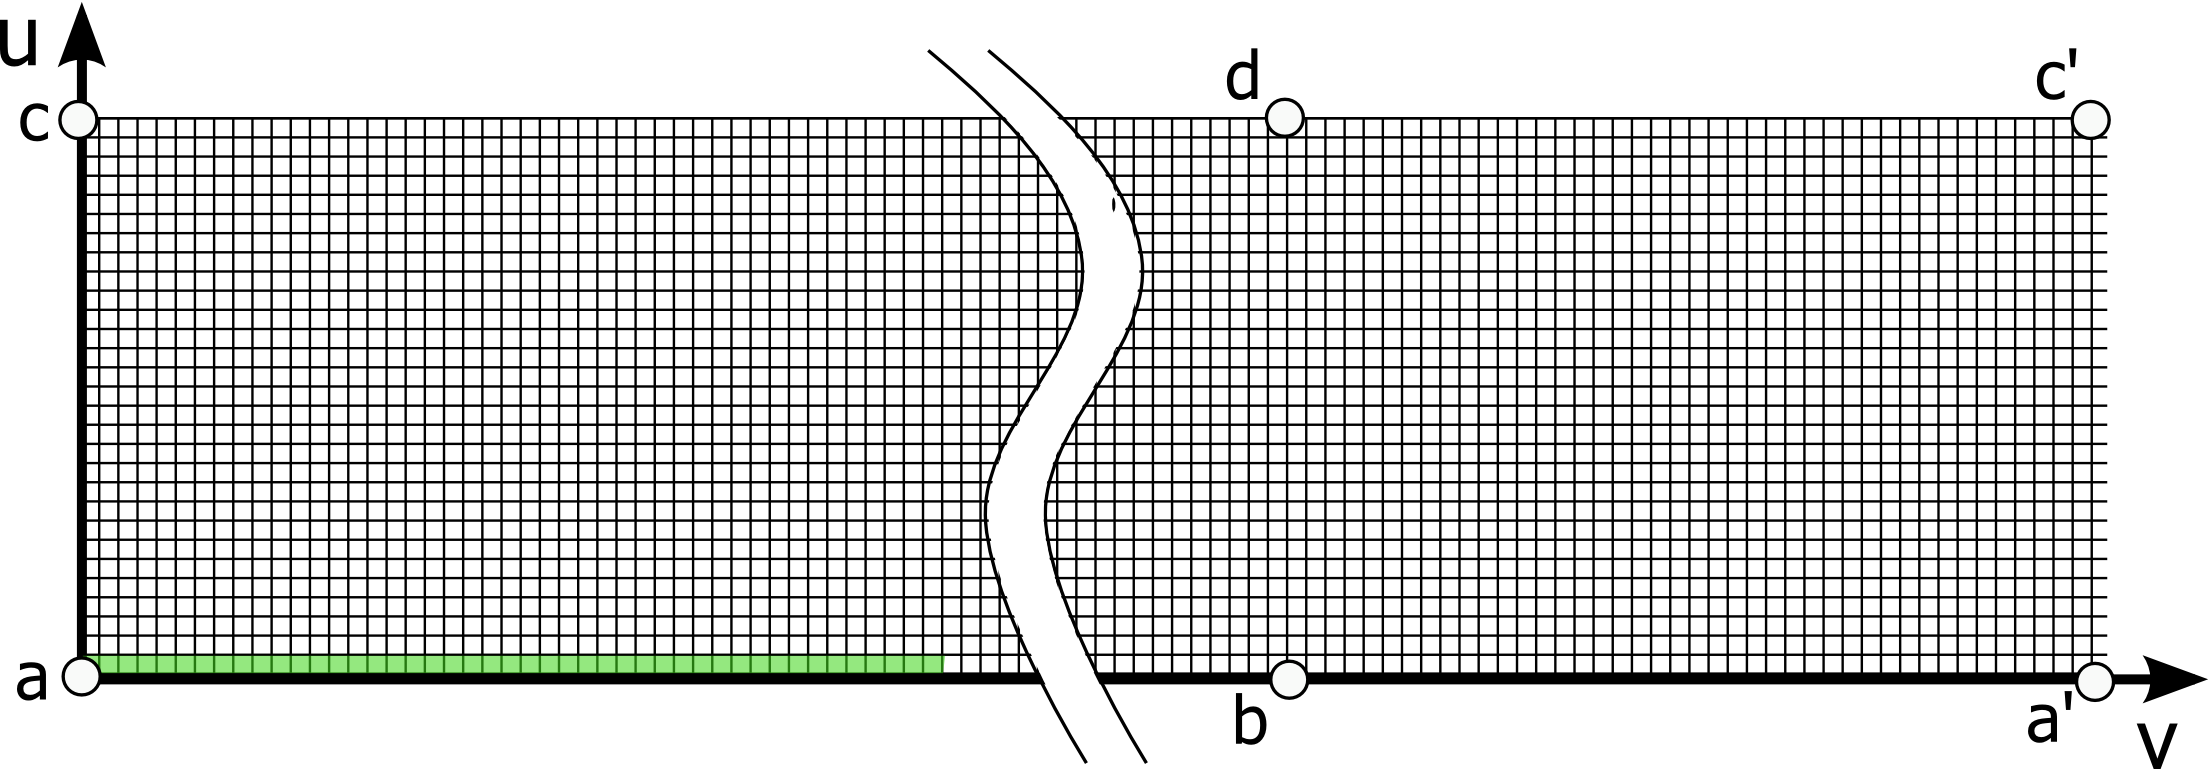
\includegraphics[width=\linewidth]{Rysunki/siatka_prostokatna.png}
	\caption{Przestrzeń obliczeniowa $(u,v)$. Węzły \textsf{a,a',b,c,c',d} odpowiadają węzłom z rys.~(\ref{fig:siatka_krzywoliniowa}). 
	\label{fig:siatka_obliczeniowa}}
\end{figure}

\indent Przyjętej w projekcie metody różnic skończonych nie da się bezpośrednio wykorzystać na siatce krzywoliniowej\footcite{Anderson, s. 170}. Wymagane jest przeprowadzenie transformacji siatki niejednorodnej do postaci prostokątnej, jak i samego równania Poissona, tak aby było spełnione w nowym układzie kartezjańskim (przekształcenie z przestrzeni fizycznej do obliczeniowej)\footcite{Blazek, s. 36}. 

\indent\newline Ogólna postać operatora laplasjanu we współrzędnych krzywoliniowych~$(u,v)$ wygląda  następująco\footnote{\url{http://www.maths.qmul.ac.uk/~wjs/MTH5102/curvcoord10.pdf}}

\begin{equation}
\nabla^2  = \frac{1}{h_1h_2}\left[\frac{\partial}{\partial u}\left(\frac{h_2}{h_1}\cdot\frac{\partial}{\partial u}\right)+\frac{\partial}{\partial v}\left(\frac{h_2}{h_1}\cdot\frac{\partial}{\partial v}\right) \right]
\end{equation}
\newline
\noindent Po wykonaniu różniczkowania wyrażeń w nawiasach okrągłych otrzymujemy jego rozwiniętą formę


\begin{equation} 
\begin{split}
\nabla^2
= 
\underbracket{\frac{1}{h_1^2}}_{A}\frac{\partial^2}{\partial u^2}
+ 
\underbracket{\frac{1}{h_2^2}}_{B}\frac{\partial^2}{\partial v^2}
& + 
\underbracket{\frac{1}{h_1h_2}\left[\frac{1}{h_1}\frac{\partial h_2}{\partial u} +  h_2\frac{\partial}{\partial u}\left(\frac{1}{h_1}\right) \right]}_{C}\frac{\partial}{\partial u}
 \\ & +
\underbracket{\frac{1}{h_1h_2}\left[ \frac{1}{h_2}\frac{\partial h_1}{\partial v}+h_1\frac{\partial}{\partial v}\left(\frac{1}{h_2}\right)\right]}_{D}\frac{\partial}{\partial v}
\end{split}
\label{eq:laplasjan_1}
\end{equation}

\noindent Występujące powyżej czynniki skalujące dane są następująco

\begin{equation}
h_1 = \sqrt{\left(\frac{\partial x}{\partial u}\right)^2+\left(\frac{\partial y}{\partial u}\right)^2}
\quad\quad\quad
h_2 = \sqrt{\left(\frac{\partial x}{\partial v}\right)^2+\left(\frac{\partial y}{\partial v}\right)^2}
\end{equation}
\newline
\noindent Pochodne czynników skalujących po współrzędnych obliczeniowych $u,v$ można wyrazić w postaci zależnej od współrzędnych z przestrzeni fizycznej $x,y$ 

\begin{equation}
\label{eq:poch_wsp_skal}
\begin{split}
\frac{\partial h_2}{\partial u} &= \frac{\partial}{\partial u}\left(\sqrt{x_v^2+y_v^2} \right)=\frac{x_v\cdot x_{uv}+y_v\cdot y_{vv}}{h_2} 
\\
\frac{\partial h_1}{\partial v} &= \frac{x_u\cdot x_{uv} + y_u\cdot y_{uv}}{h_1} 
\\
\frac{\partial}{\partial u}\left(\frac{1}{h_1}\right)&=\frac{\partial}{\partial u}\left(\frac{1}{\sqrt{x_u^2+y_u^2}}\right)= - \frac{x_u\cdot x_{uu} + y_u\cdot y_{uu}}{h_1^3}
\\
\frac{\partial}{\partial v}\left(\frac{1}{h_2}\right)&=-\frac{x_v\cdot x_{vv}+y_v\cdot y_{vv}}{h_2^3}
\end{split}
\end{equation}
\newline
\noindent Do obliczenia wartości poszczególnych pochodnych cząstkowych współrzędnych $x = x(u,v), y = y(u,v)$ po $u,v$ niezbędne jest użycie metody różnic skończonych.

\section{Dyskretyzacja metodą różnic skończonych}
\indent\indent W metodzie różnic skończonych operatory różniczkowania zastępowane są odpowiednimi operatorami różnicowymi. W rezultacie otrzymuje się układ równań algebraicznych, który w przeciwieństwie do układu równań różniczkowych jest prostszy i w większości przypadków w ogóle możliwy do rozwiązania. Otrzymany wynik jest jednak rozwiązaniem przybliżonym, o błędzie zależnym od wybranego rodzaju schematu różnicowego. Przybliżenie pochodnej różnicą centralną daje błąd o rząd mniejszy niż w przypadku różnicy w przód lub wstecznej, tzn. ma błąd obcięcia $\mathcal{O}(\Delta x)^2$. Fakt ten przemawia za użyciem jej w projekcie\footcite{Anderson, s. 132}.

\begin{figure}[H]
	\centering
    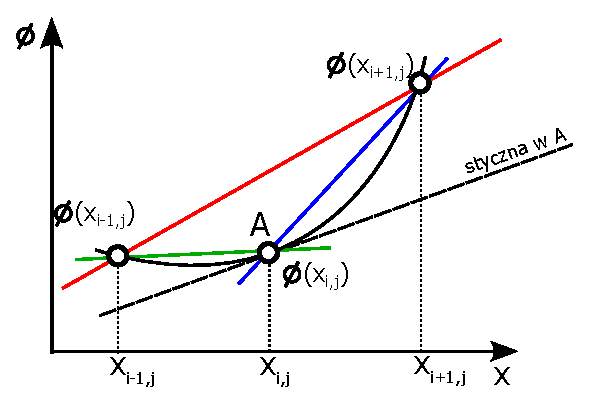
\includegraphics[width=0.6\linewidth]{Rysunki/roznice_skonczone_interpretacja.eps}
  \caption{Interpretacja geometryczna różnic skończonych: \color{blue}{przedniej}, \color{green}{wstecznej} \color{black}{oraz} \color{red}{centralnej} \color{black} wyraźnie wskazuje na przewagę tej ostatniej pod względem wielkości błędu popełnianego przy dyskretyzacji pochodnej.
	\label{fig:roznice_interpretacja}}
\end{figure}

\noindent Poniżej użyto oznaczeń $h_u, h_v$ na wartości kroku siatki odpowiednio na kierunku osi $Ou$ oraz $Ov$. \newline

\noindent Różnice dla pochodnych pierwszego rzędu:

\[
x_u = \frac{x_{i+1,j}-x_{i-1,j}}{2h_u} \quad\quad
 x_v = \frac{x_{i,j+1}-x_{i,j-1}}{2h_v}
\]

\begin{figure}[H]
	\centering
    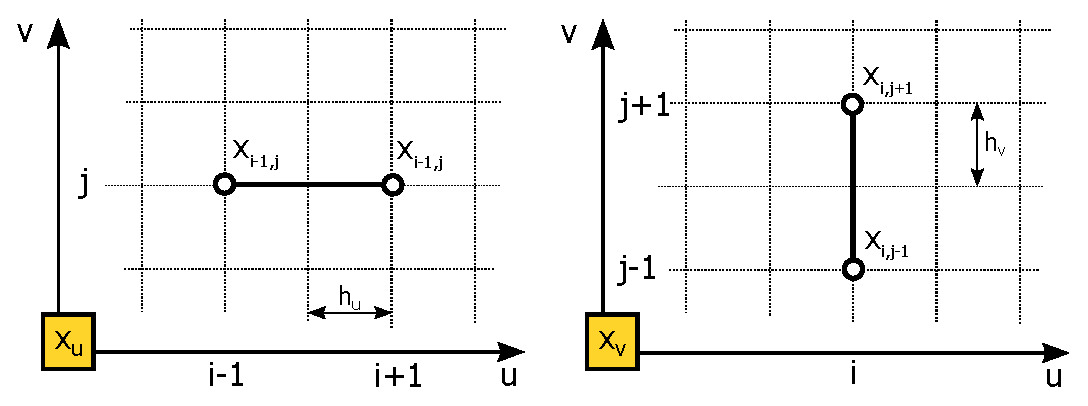
\includegraphics[width=\linewidth]{Rysunki/roznice_skonczone_x.eps}
	\caption{Konstrukcja różnic skończonych drugiego rzędu zmiennej \mbox{$x=x(u,v)$}
	\label{fig:roznice_skonczone_x}}
\end{figure}

\noindent Konstrukcja różnic dla $y_u, y_v$ jest analogiczna

\[
y_u = \frac{y_{i+1,j}-y_{i-1,j}}{2h_u} \quad y_v = \frac{y_{i,j+1}-y_{i,j-1}}{2h_v}
\]

\noindent Różnice dla pochodnych drugiego rzędu (rys.~\ref{fig:roznice_skonczone_xx}):

\[
x_{uu} = \frac{x_{i+1,j}-2x_{i,j}+x_{i-1,j}}{h_u^2} \quad x_{uv} = \frac{x_{i+1,j+1}-x_{i+1,j-1}-x_{i-1,j+1}+x_{x-1,j-1}}{4h_uh_v}
\]

\[
y_{uu} = \frac{y_{i+1,j}-2y_{i,j}+y_{i-1,j}}{h_u^2} \quad y_{uv} = \frac{y_{i+1,j+1}-y_{i+1,j-1}-y_{i-1,j+1}+y_{i-1,j-1}}{4h_uh_v}
\]


\begin{figure}[H]
	\centering
    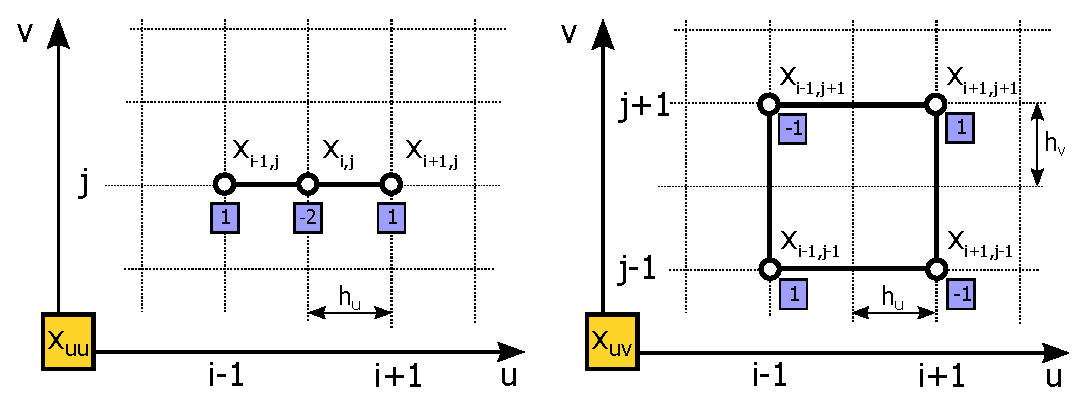
\includegraphics[width=\linewidth]{Rysunki/roznice_skonczone_xx.eps}
	\caption{Konstrukcja różnic skończonych drugiego rzędu dla zmiennej $x=x(u,v)$
	\label{fig:roznice_skonczone_xx}}
\end{figure}

\noindent Dla uproszczenia dalszego zapisu wprowadźmy następujące oznaczenie na wartość zmiennej $\phi$ w węźle o współrzędnych $(u_i,v_i)$:

\[
\phi(u_i, v_j) \triangleq \phi_{i,j}
\]

\noindent Wstawiając powyższe różnice do \ref{eq:poch_wsp_skal}, oraz analogicznie konstruując różnice dla zmiennej $\phi$, po wstawieniu otrzymanych związków do wzoru na laplasjan we współrzędnych obliczeniowych \ref{eq:laplasjan_1} otrzymujemy 
\begin{equation}
\begin{split}
A\cdot\frac{\phi_{i+1,j}-2\phi_{i,j}+\phi_{i-1,j}}{h_u^2}+B\cdot\frac{\phi_{i,j+1}-2\phi_{i,j}+\phi_{i,j-1}}{h_v^2}&+ \\ C\cdot\frac{\phi_{i+1,j}-\phi_{i-1,j}}{2h_v}+D\cdot\frac{\phi_{i,j+1}-\phi_{i,j-1}}{2h_v}&=-1
\end{split}
\end{equation}
\newpage \noindent Ostatecznie po uporządkowaniu względem $\phi$ równanie Poissona w postaci różnicowej wygląda następująco:
\begin{equation}
\begin{split}
\underbracket{\left(\frac{B}{h_v^2}-\frac{D}{2h_v}\right)}_{a}\phi_{i,j-1}\;&+\;\underbracket{\left(\frac{A}{h_u^2}-\frac{C}{2h_u}\right)}_{b}\phi_{i-1,j} \;\underbracket{-2\left(\frac{A}{h_u^2}+ 
\frac{B}{h_v^2}\right)}_{c}\phi_{i,j}\;+ \\ &+\; \underbracket{\left(\frac{A}{h_v^2} + \frac{C}{2h_u}\right)}_{d}\phi_{i+1,j}\;+\; \underbracket{\left(\frac{B}{h_v^2}+\frac{D}{2h_v}\right)}_{e}\phi_{i,j+1}=-1
\end{split}
\label{eq:poisson_roznicowo}
\end{equation}
\newline
\noindent Przedstawienie go w takiej formie umożliwia łatwe zapisanie układu równań dla całego obszaru obliczeniowego. Wzajemne rozmieszczenie przestrzenne węzłów odpowiadających poszczególnym wartościom zmiennej $\phi$, tworzących tzw. pięciopunktową gwiazdę różnicową (ang. \textit{five-point-star}), zaprezentowano na rys.~\ref{fig:wezly}.

\begin{figure}[h]
  \centering
    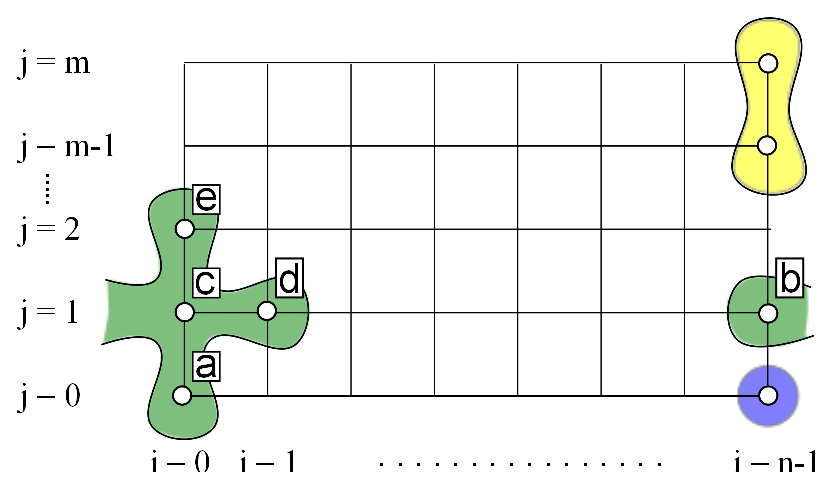
\includegraphics[scale=0.8]{Rysunki/gwiazda_roznicowa.eps}
  \caption{Siatka z wyróżnionymi węzłami, tworzącymi pięciopunktową \colorbox{green!70!blue!30}{gwiazdę różnicową} oraz warunki brzegowe: \colorbox{blue!30}{Dirichleta} i \colorbox{yellow!50}{Neumanna}.
  \label{fig:wezly}}
\end{figure}

\section{Warunki brzegowe}
\indent\indent Układ równań utworzony na podstawie wzoru \ref{eq:poisson_roznicowo} należy uzupełnić o poniższe warunki brzegowe (rys.~\ref{fig:wezly}).
\begin{enumerate}
\item \textbf{warunek ciągłości} - węzły leżące na lewej i prawej krawędzi siatki są w rzeczywistości węzłami sąsiadującymi ze sobą. W równaniu~\ref{eq:poisson_roznicowo} zapisanym dla węzła tego rodzaju wartość współczynnika \textsf{b} (lub odpowiednio~\textsf{d}) pochodzi z węzła leżącego na samym końcu (początku) tego samego rzędu siatki.
\item \textbf{warunek Dirichleta} - zerowa wartość zmiennej $\phi$ na krawędzi profilu
\begin{equation}
\phi\big|_{\partial S} = \phi_{i,0} = 0
\end{equation}
\item \textbf{warunek Neumanna} - zerowa wartość pochodnej $\phi$ w kierunku normalnym do zewnętrznego brzegu obszaru obliczeniowego \begin{equation}
\frac{\partial\phi}{\partial n}=0 \iff \frac{\phi_{i,m}-\phi_{i,m-1}}{h_v}=0
\end{equation}
gdzie: $m$ - indeks zewnętrznego rzędu siatki
\end{enumerate}

\section{Rozwiązanie zagadnienia}

\indent\indent Rozwiązanie uprzednio zdefiniowanego zagadnienia sprowadza się do rozwiązania macierzowego układu równań o postaci
\begin{equation}
\left[\mathbb{K}\right]\{\phi\}=\{f\}
\end{equation}
\noindent gdzie:
\begin{description}\addtolength{\itemsep}{-1.5\baselineskip}
  \item[\quad]$\mathbb{K}$ - macierz współczynników
  \item[\quad]$\{\phi\}$ - wektor poszukiwanych wartości funkcji $\phi$
  \item[\quad]$\{f\}$ - wektor prawej strony
\end{description}
\noindent W rozwiniętej formie równanie prezentuje się następująco (puste miejsca oznaczają zerowe elementy)

\begin{equation}
\begin{bmatrix}
      1 &   & 											\\[0.8pt]
        & 1 & 											\\[0.8pt]
        &   & \ddots 									\\[0.8pt]       
        &   &   & 1 									\\[0.8pt]           
      a &   &   &   & c & d &   & b & e 				\\[0.8pt]
        & a &   &   & b & c & d &   &   & e	    		\\[0.8pt]
        &&\ddots&&&\ddots&\ddots&\ddots&&&\ddots	   	\\[0.8pt]
        &   &   & a &   &   & b & c & d &   &   & e 	\\[0.8pt]
        &   &   &   & a & d &   & b & c &   &   &   & e \\[0.8pt]
        &   &   &   &   & -1&   &   &   & 1 &   &   &   \\[0.8pt]
        &   &   &   &   &   & -1&   &   &   & 1 &   &   \\[0.8pt]
        &   &   &   &   &   &  &\ddots &&   &&\ddots&   \\[0.8pt]
        &   &   &   &   &   &   &   & -1&   &   &   & 1 \\[0.8pt]
\end{bmatrix}
\begin{bmatrix}
	\phi_{0,0} 		\\[0.8pt]
	\phi_{1,0} 		\\[0.8pt]
		\vdots 		\\[0.8pt]
	\phi_{n-1,0} 	\\[0.8pt]
	\phi_{0,1} 		\\[0.8pt]
	\phi_{1,1} 		\\[0.8pt]
		\vdots 		\\[0.8pt]
	\phi_{n-2,1} 	\\[0.8pt]
	\phi_{n-1,1} 	\\[0.8pt]
	\phi_{0,m} 		\\[0.8pt]
	\phi_{1,m} 		\\[0.8pt]
		\vdots 		\\[0.8pt]
	\phi_{n-1,m}	\\[0.8pt]	
\end{bmatrix}
=
\begin{bmatrix}
	0 \\[0.8pt]
	0 \\[0.8pt]
	0 \\[0.8pt]
	0 \\[0.8pt]
   -1 \\[0.8pt]
   -1 \\[0.8pt]
   -1 \\[0.8pt]
   -1 \\[0.8pt]
   -1 \\[0.8pt]
   -1 \\[0.8pt]
	0 \\[0.8pt]
	0 \\[0.8pt]
	0 \\[0.8pt]
	0 \\[0.8pt]
\end{bmatrix}
\label{eq:poisson_macierz}
\end{equation}

\indent Macierz współczynników ma rozmiar $(n\cdot m)\times (n\cdot m)$, gdzie $n$ - liczba węzłów na profilu, $m$ - liczba rzędów siatki. Jej struktura jest charakterystyczna dla zagadnień opisanych równaniami różniczkowymi cząstkowymi, tzn. większość jej elementów jest  zerowa. Macierze o powyższej własności nazywane są rzadkimi (ang. \textit{sparse}) \footcite{Saad,s. 67}. Dla rozważanego w niniejszym projekcie problemu rozmiar macierzy wynosi $N\times N = 12\;524\times 12\;524 = 156\;850\;576$ elementów, z czego tylko $0{,}03\%$ ma niezerowe wartości\footnote{Macierz współczynników zawiera po $n$ wartości wynikających z warunków brzegowych Dirichleta i Neumanna, oraz $5n(m-2)$ z zapisu różnicowego równania Poissona. Procentowe wypełnienie macierzy można obliczyć następująco: $\frac{5n(m-2)+n+n}{n^2m^2}\approx\frac{5}{nm}$}. 

\indent Do rozwiązania układu \ref{eq:poisson_macierz} zdecydowano się na skorzystanie ze stabilizowanej metody wzajemnie sprzężonych gradientów BiCGSTAB (ang. \textit{BiConjugate Gradient STABilized method}). Jest to metoda iteracyjna, oparta na podprzestrzeniach Kryłowa, odpowiednia do zagadnień dobrze uwarunkowanych, z macierzami rzadkimi \footcite{Blazek,s. 208}. Za jej wykorzystaniem przemawia również dostępność implementacji w bibliotece Eigen (patrz podrozdział \ref{sec:bibl_zewn}).

\noindent Tolerancja rozwiązania została przyjęta na poziomie tolerancji danych wejściowych, tzn. $\epsilon = 10^{-6}$.




\indent W wyniku rozwiązania układu \ref{eq:poisson_macierz} otrzymuje się wartości $\phi$ wyrażone w przestrzeni obliczeniowej. Aby móc skorzystać ze wzoru na odległość~\ref{eq:d_1} należy rozwiązać pomocniczy układ równań wynikający wprost z reguły łańcuchowej \ref{eq:chain_rule}, mnożąc obie strony przez odwrotność macierzy Jacobiego.

\begin{equation}
\begin{cases}
	\phi_u = \phi_x\cdot x_u + \phi_y\cdot y_u \\
	\phi_v = \phi_x\cdot x_v + \phi_y\cdot y_v
\end{cases} \iff
\begin{bmatrix}
\phi_u \\ \phi_v
\end{bmatrix}=
\underbracket{\begin{bmatrix}
x_u && y_u \\
x_v && y_v
\end{bmatrix}}_{\text{macierz Jacobiego}}
\begin{bmatrix}
\phi_x \\ \phi_y
\end{bmatrix}
\label{eq:chain_rule}
\end{equation}

\begin{equation}
\begin{bmatrix}
\phi_x \\ \phi_y
\end{bmatrix} = 
\begin{bmatrix}
x_u && y_u \\
x_v && y_v
\end{bmatrix}^{-1}
\begin{bmatrix}
\phi_u \\ \phi_v
\end{bmatrix}
\label{eq:jakobian}
\end{equation}

\noindent\newline Szukana zależność transformacyjna \ref{eq:jakobian} wymaga dyskretyzacji pochodnych cząstkowych według przedstawionego wcześniej schematu różnicowego.

\[
\phi_u = \frac{\phi_{i+1,j}-\phi_{i-1,j}}{2h_u} \quad \phi_v = \frac{\phi_{i,j}-\phi_{i,j-1}}{h_v}
\]
	\chapter{Implementacja}

\indent 


\section{Układ logiczny programu}

\indent\indent Funkcjonalność programu została podzielona między klasy \textsf{cGrid, cSolution} oraz \textsf{cSolver}. Pierwsza z nich przechowuje wygenerowaną siatkę obliczeniową, druga otrzymane rozwiązanie, natomiast  ostatnia z nich jest klasą nadrzędną, z jej poziomu wywoływane są wszystkie operacje przewidziane w funkcjonalności programu. 

\section{Biblioteki zewnętrzne}\label{sec:bibl_zewn}

\indent\indent Do operacji na macierzach wykorzystano darmową bibliotekę języka C++ Eigen (wersja 3.1.2). Za jej wyborem do niniejszego projektu przemawia niezawodność i szybkość operacji na macierzach dowolnych rozmiarów, oraz zaimplementowanie metod do rozwiązania rzadkich układów macierzowych\footnote{\url{http://eigen.tuxfamily.org/}}.

\section{Klasa cGrid}

\indent\indent Przechowuje węzły siatki oraz umożliwia do nich dostęp. Do przechowywania węzłów posłużono się kontenerem \textsf{vector} zaimplementowanym w bibliotece standardowej języka C++.

\begin{lstlisting}[style = nonumbers]
	std::vector<cPoint> mPoints;	
\end{lstlisting}

\noindent W przeciwieństwie do dwuwymiarowej struktury siatki sam kontener przechowuje elementy w porządku liniowym, co wymusza dodanie operatora dostępu do elementu (węzła) o indeksach $(i,j)$.
\begin{lstlisting}[style = nonumbers]
	cPoint & operator()(const int i, const int j)
\end{lstlisting}
\noindent Dodawanie węzłów do kontenera odbywa się przy pomocy metody 
\begin{lstlisting}[style = nonumbers]
	void	addNode(const cPoint & inPoint, eGridMode mode = GRID)	
\end{lstlisting}	
gdzie oprócz referencji do węzła przekazuje się jego typ \textsf{GRID / PROFILE}. Jest to o tyle ważne, ponieważ dodanie węzła profilu zwiększa wartość wewnętrznego licznika, na podstawie którego jest generowana siatka i przeprowadzane rozwiązanie metodą siłową.

\noindent Poniższe metody dostępowe zwracają odpowiednio liczbę węzłów \newline (\textsf{GRID} - siatki, \textsf{PROFILE} - na profilu) oraz rzędów siatki
\begin{lstlisting}[style = nonumbers]
	int	nodeCount(eGridMode mode = GRID) const	
	int	rowCount() const;
\end{lstlisting}	

\section{Klasa cSolution}

\indent\indent Publiczna klasa dziedziczona po klasie \textsf{cGrid}, oprócz obiektu siatki dodatkowo przechowuje w kontenerze typu \textsf{vector} wartości obliczonego rozwiązania zagadnienia. Poniższa metoda dodaje do kontenera wartość \textsf{inValue} typu (\textsf{DISTANCE, PHI})

\begin{lstlisting}[style = nonumbers]
	void	addValue(double inValue, eSolutionData valueType= DISTANCE);	
\end{lstlisting}
Analogicznie zwrot zapisanych wartości uzyskuje się korzystając z metody

\begin{lstlisting}[style = nonumbers]
	double	getValue(int k, eSolutionData valueType = DISTANCE);
\end{lstlisting}
gdzie $k$ jest bezwzględnym numerem węzła 


\section{Klasa cSolver}

\indent\indent Nadrzędna klasa programu będąca jego interfejsem. Przechowuje obiekt \textsf{mSolution} typu \textsf{cSolution} oraz obiekty klasy \textsf{Eigen}, które wykorzystywane są do rozwiązania układu macierzowego:

\begin{lstlisting}[style = nonumbers]
	//Macierz wsp'ó''ł'czynnik'ó'w
	Eigen::SparseMatrix<double>		K;
	
	//Wektor prawej strony		
	Eigen::VectorXd					f;	
	
	//Wektor rozwi'ą'zania		
	Eigen::VectorXd					x;	
		
	//Obiekt rozwi'ą'zuj'ą'cy uk'ł'ad			 
	Eigen::BiCGSTAB<Eigen::SparseMatrix<double>>	solver;		
\end{lstlisting}



\subsection{Metody prywatne}

\noindent Metoda implementująca rozwiązanie siłowe
\begin{lstlisting}[style = nonumbers]
	void	solveBruteForce()		
\end{lstlisting}
\color{white}{.}\color{black}{}		%Sztuczny odstęp

\noindent Metoda implementująca rozwiązanie równaniem Poissona
\begin{lstlisting}[style = nonumbers]
	void	solvePoisson()		
\end{lstlisting}
\color{white}{.}\color{black}{}		%Sztuczny odstęp

\noindent Metoda bezpośrednio wyznaczająca odległość między węzłami
\begin{lstlisting}[style = nonumbers]
	double	distanceBetween(cPoint & p_1, cPoint & p_2)
\end{lstlisting}
\vspace*{-.5cm}
\begin{enumerate} \itemsep1pt \parskip0pt \parsep0pt
	\item[-] \textsf{argumenty:} 
	\item[] p\_1 - referencja do pierwszego węzła
	\item[] p\_2 - referencja do drugiego węzła
	\item[-] \textsf{zwraca:} odległość $d(p_1,p_2)$	
\end{enumerate}

\noindent Metoda wyznaczająca odległość na postawie wzoru \ref{eq:jakobian}
\begin{lstlisting}[style = nonumbers]
	void	computeDistance()	
\end{lstlisting}
\color{white}{.}\color{black}{}		%Sztuczny odstęp

\noindent Metoda obliczająca pochodne cząstkowe dla danego węzła siatki
\begin{lstlisting}[style = nonumbers]
	double	partial(int k, ePartial partial);
\end{lstlisting}
\vspace*{-.5cm}
\begin{enumerate} \itemsep1pt \parskip0pt \parsep0pt
	\item[-] \textsf{argumenty:} 
	\item[] k - bezwzględny numer węzła 
	\item[] partial - rodzaj pochodnej ($x_u, x_v, y_u, y_v, x_{uu}, x_{uv}, x_{vv}, y_{uu}, y_{uv}, y_{vv}$)
	\item[-] \textsf{zwraca:} wartość pochodnej	
\end{enumerate}




\subsection{Metody publiczne}
\noindent Metoda wczytująca do pamięci współrzędne węzłów profilu
\begin{lstlisting}[style = nonumbers]
	void	addProfile(std::string filePath)
\end{lstlisting}
\vspace*{-.5cm}
\begin{enumerate} \itemsep1pt \parskip0pt \parsep0pt
	\item[-] \textsf{argument:} ścieżka do pliku z danymi wejściowymi\newline	
\end{enumerate}

\noindent Metoda generująca siatkę obliczeniową wokół profilu
\begin{lstlisting}[style = nonumbers]
	void	generateGrid(cPoint & circleCenter,
						 double circleRadius,
						 int linesDensity)
\end{lstlisting}
\vspace*{-.5cm}
\begin{enumerate} \itemsep1pt \parskip0pt \parsep0pt
	\item[-] \textsf{argumenty:} 
	\item[] circleCenter - punkt środka siatki
	\item[] circleRadius - promień siatki
	\item[] linesDensity - ilość rzędów siatki\newline		
\end{enumerate}

\noindent Metoda rozwiązująca zagadnienie
\begin{lstlisting}[style = nonumbers]
	double	solve(eSolutionType type = POISSON)	
\end{lstlisting}
\vspace*{-.5cm}
\begin{enumerate} \itemsep1pt \parskip0pt \parsep0pt
	\item[-] \textsf{argumenty:}
	\item[] type - rodzaj używanej metody (POISSON, BRUTE FORCE)
	\item[-] \textsf{zwraca:} czas wykonania w sekundach\newline	
\end{enumerate} 

\noindent Metoda zapisująca rozwiązanie do pliku
\begin{lstlisting}[style = nonumbers]
	void	saveSolution(eSolutionData dataType = DISTANCE,
	                     std::string filePath = "solution.dat",  
	                     eFileExtension extension = TECPLOT)	
\end{lstlisting}
\vspace*{-.5cm}
\begin{enumerate} \itemsep1pt \parskip0pt \parsep0pt
	\item[-] \textsf{argumenty:}
	\item[] dataType - rodzaj zapisywanej danej, domyślnie odległość
	\item[] filePath - ścieżka i nazwa pliku wynikowego
	\item[] extension - opcjonalne dodanie nagłówka programu Tecplop\newline
\end{enumerate} 


	\chapter{Wyniki}

\indent\indent Przeprowadzono uruchomienie programu dla dwóch profili lotniczych: symetrycznego \textsf{NACA 0012} oraz \textsf{NACA 8207}. Współrzędne punktów tworzących ich obrysy zaczerpnięto ze strony internetowej \url{http://www.ae.illinois.edu/m-selig/ads/coord_database.html}. Ze względu na użycie w projekcie naiwnego sposobu generowania siatki obliczeniowej, o jednorodnym odstępie między węzłami w kierunku $v$, zdecydowano się na zagęszczenie siatki do stu rzędów. Do celów porównawczych dla każdego z przypadków przeprowadzono obliczenia metodą siłową. Otrzymane pliki wyjściowe \textsf{.dat} wczytano do programu \textsf{Tecplot}, a wygenerowane mapy konturowe przedstawiono poniżej na rysunkach. Na końcu rozdziału zaprezentowano wykresy obliczonej odległości dla pierwszego rzędu siatki.

%Rysunki całego obszaru obliczeniowego NACA 0012
\begin{figure}[h]	
    \begin{subfigure}[h]{\textwidth}
    	\centering
    	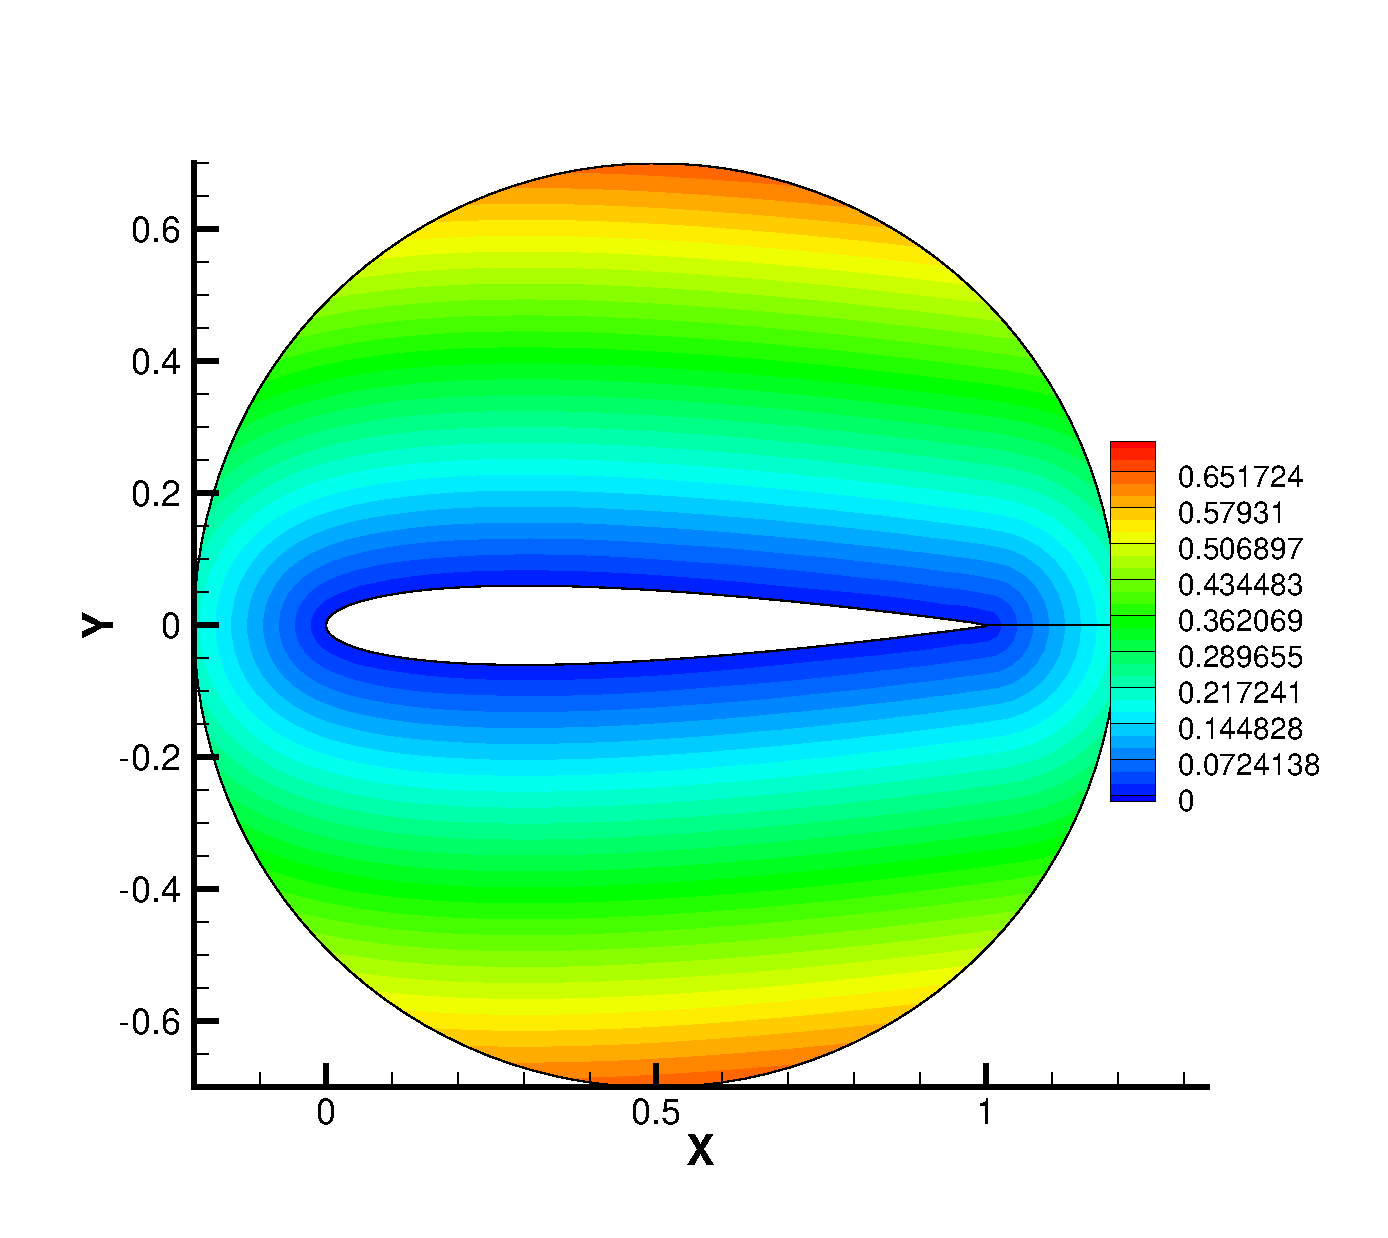
\includegraphics[trim = 22mm 10mm 10mm 20mm, width=0.9\linewidth]{Rysunki/NACA_0012_profil_brute.eps}
    	\subcaption{Metoda siłowa}	    	
	\end{subfigure}    
	\begin{subfigure}[h]{\textwidth}
		\centering
    	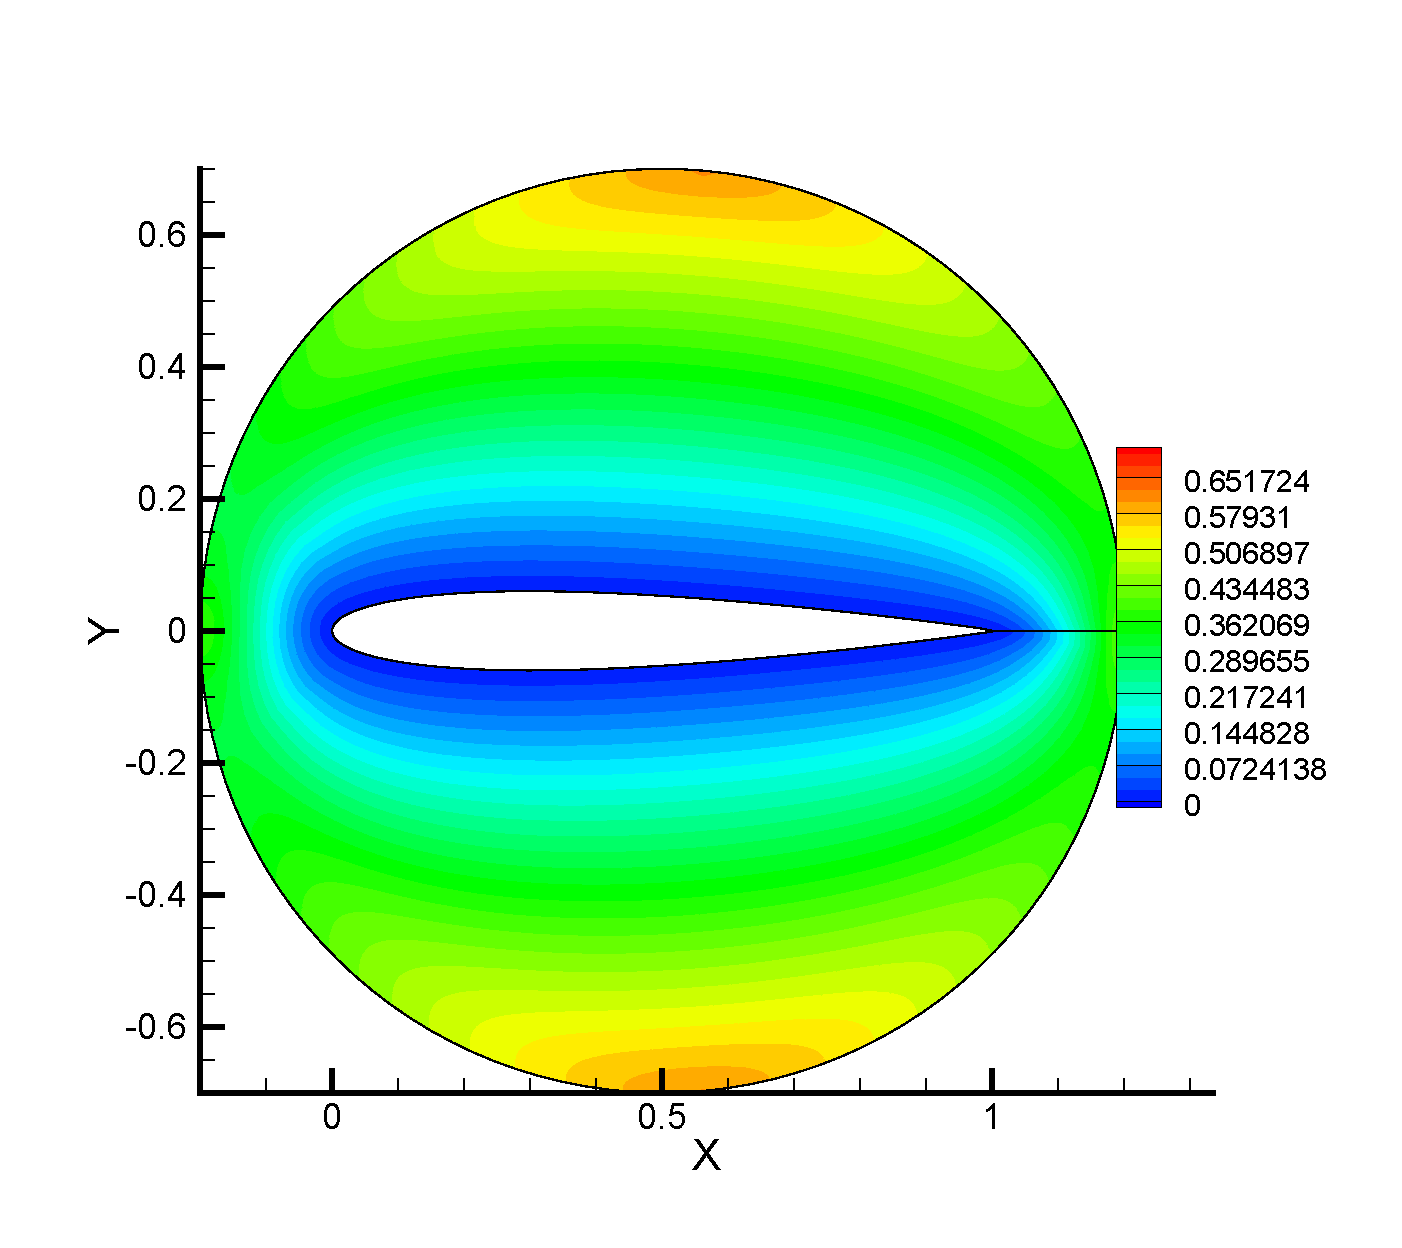
\includegraphics[trim = 22mm 10mm 10mm 20mm, width=0.9\linewidth]{Rysunki/NACA_0012_profil_poisson.eps}      	
    	\subcaption{Metoda Poissona}
	\end{subfigure}
	\caption{Profil NACA 0012}
\end{figure}

\begin{figure}[h]	
    \begin{subfigure}[h]{\textwidth}
    	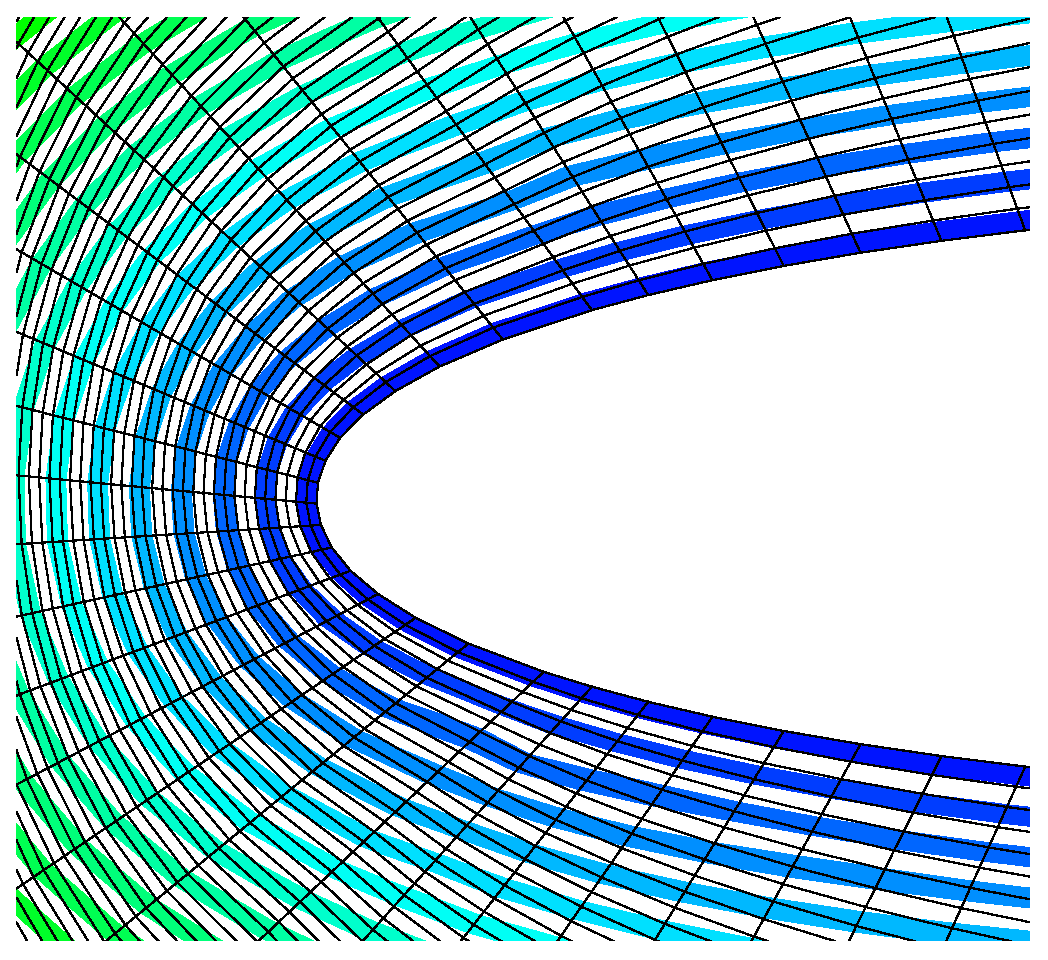
\includegraphics[width=0.5\textwidth]{Rysunki/NACA_0012_nosek_brute}  
    	\quad      
    	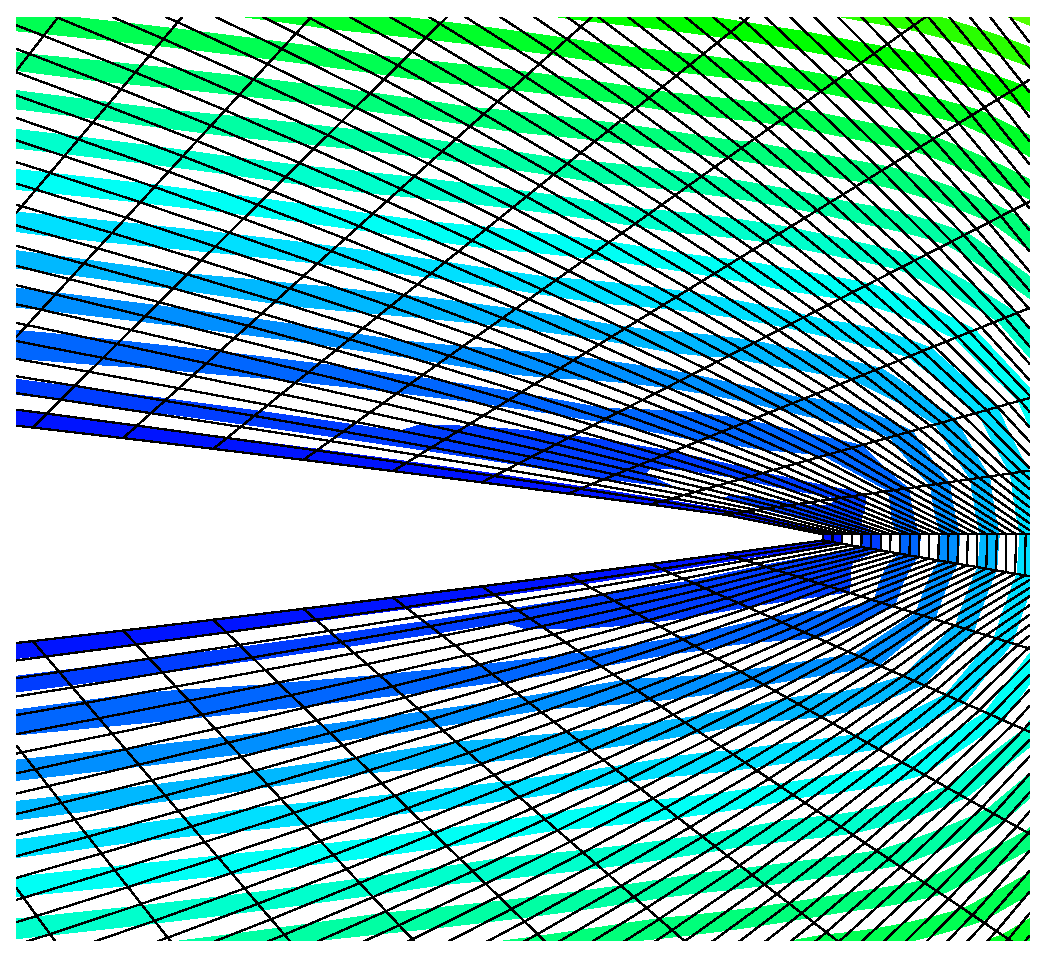
\includegraphics[width=0.5\textwidth]{Rysunki/NACA_0012_ostrze_brute}
    	\subcaption{Metoda siłowa}
    	\vspace{1cm}
	\end{subfigure}
	    
	\begin{subfigure}[h]{\textwidth}
    	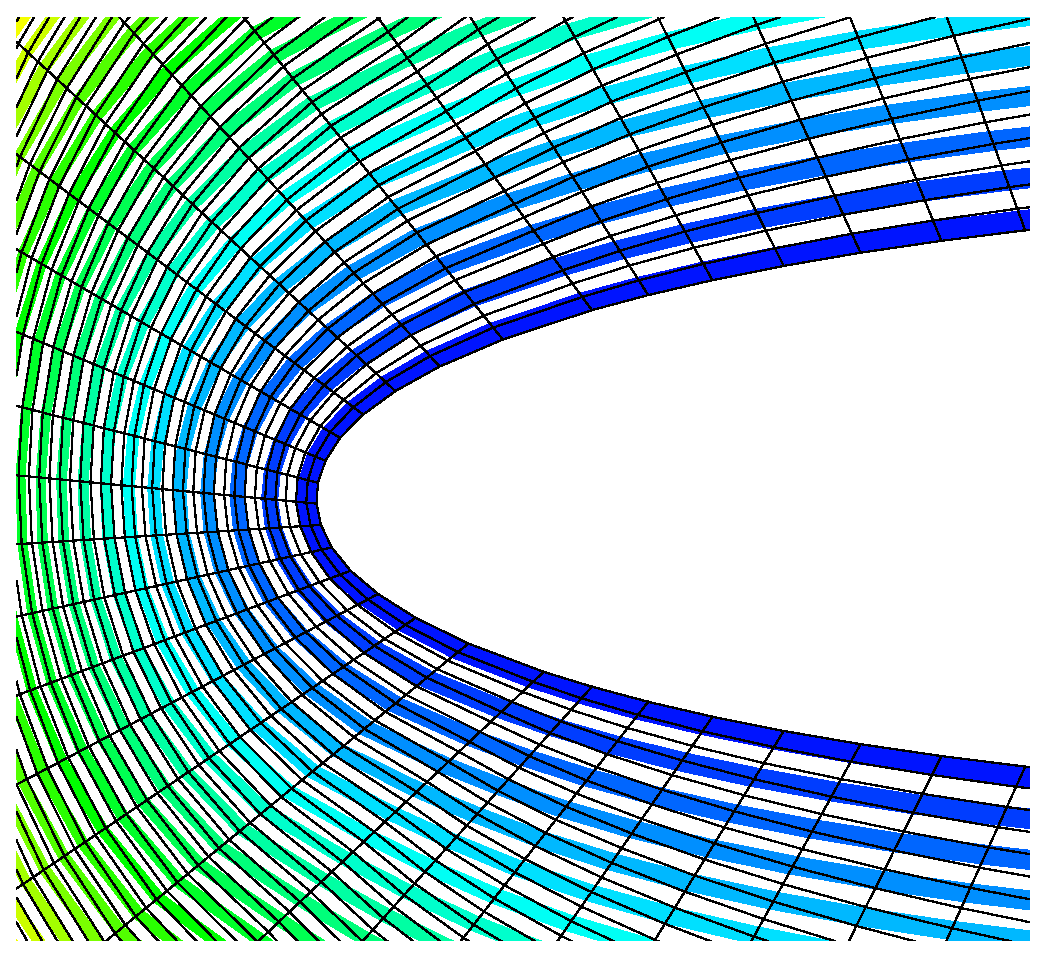
\includegraphics[width=0.5\textwidth]{Rysunki/NACA_0012_nosek_poisson}  
    	\quad      
    	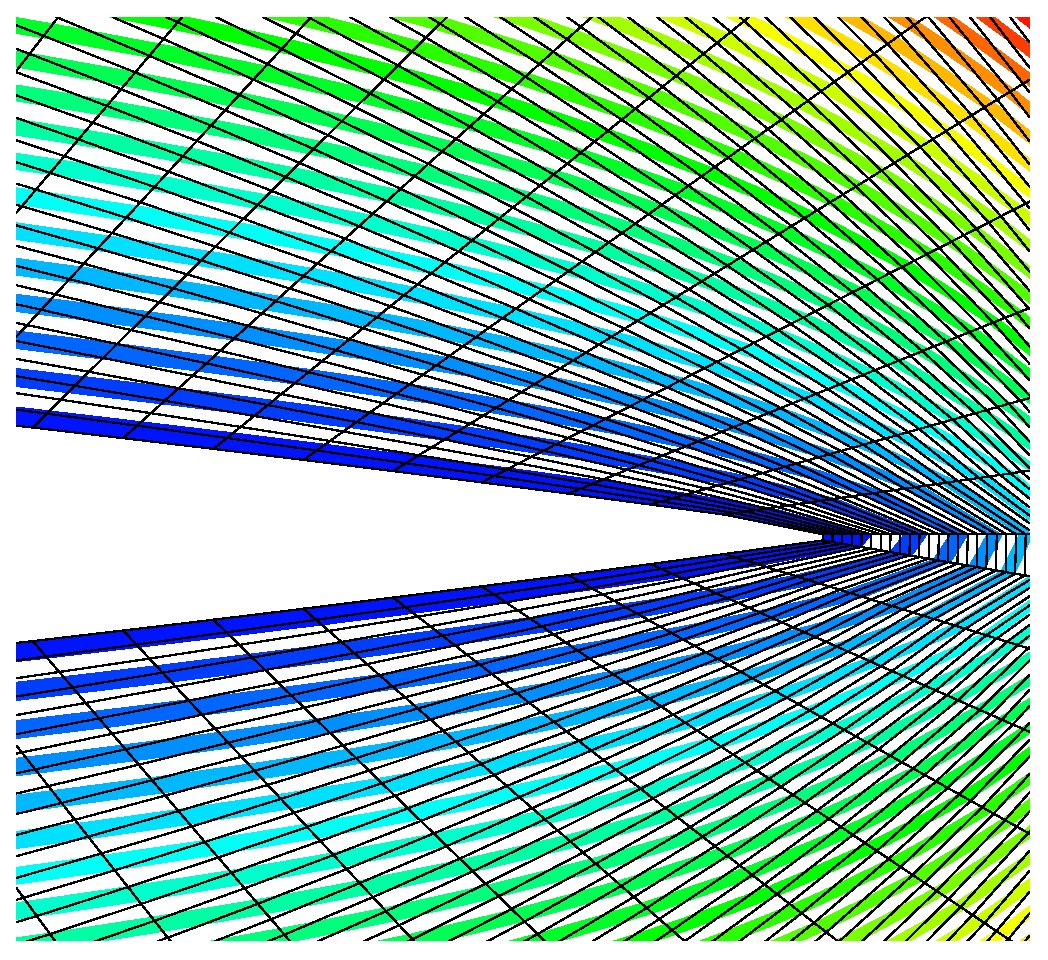
\includegraphics[width=0.5\textwidth]{Rysunki/NACA_0012_ostrze_poisson}		
		\subcaption{Metoda Poissona}
	\end{subfigure}
	\caption{Profil NACA 0012 (po lewej nosek profilu, po prawej ostrze)}
\end{figure}

%Rysunki całego obszaru obliczeniowego NACA 8207
\begin{figure}[h]	
    \begin{subfigure}[h]{\textwidth}
    	\centering
    	\includegraphics[trim = 22mm 10mm 10mm 20mm, width=0.9\linewidth]{Rysunki/NACA_8207_profil_brute}
    	\subcaption{Metoda siłowa}	    	
	\end{subfigure}    
	\begin{subfigure}[h]{\textwidth}
		\centering
    	\includegraphics[trim = 22mm 10mm 10mm 20mm, width=0.9\linewidth]{Rysunki/NACA_8207_profil_poisson}      	
    	\subcaption{Metoda Poissona}
	\end{subfigure}
	\caption{Profil NACA 8207}
\end{figure}

\begin{figure}[h]	
    \begin{subfigure}[h]{\textwidth}
    	%\centering
    	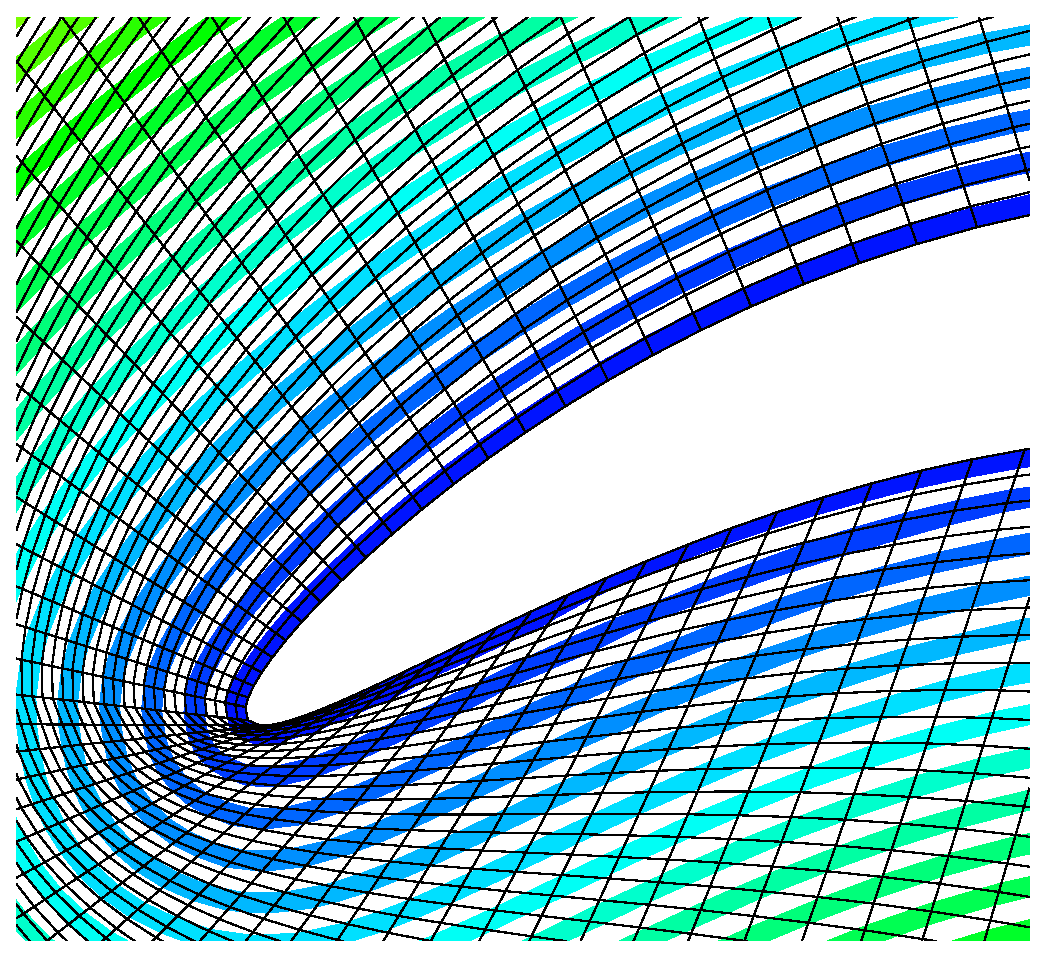
\includegraphics[width=0.5\textwidth]{Rysunki/NACA_8207_nosek_brute}  
    	\quad      
    	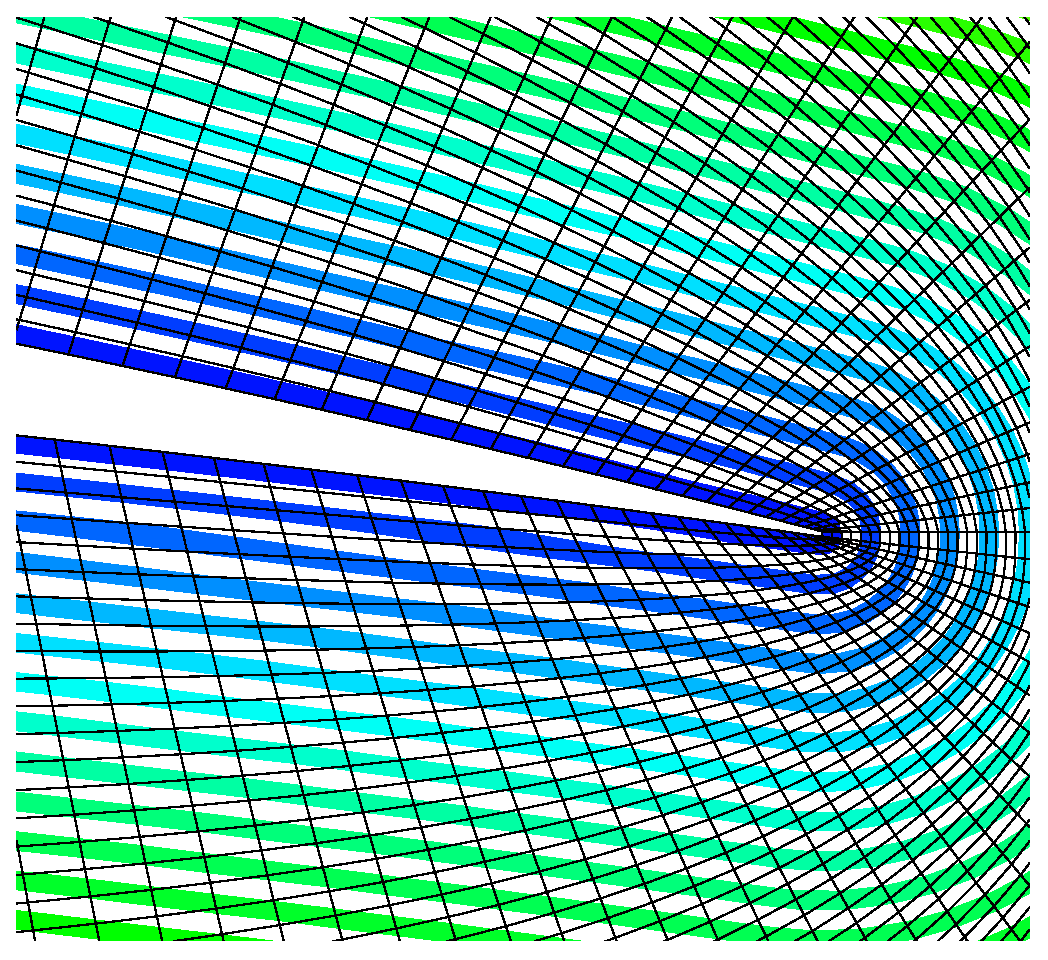
\includegraphics[width=0.5\textwidth]{Rysunki/NACA_8207_ostrze_brute}
    	\subcaption{Metoda siłowa}
    	\vspace{1cm}
	\end{subfigure}
    
	\begin{subfigure}[h]{\textwidth}
    	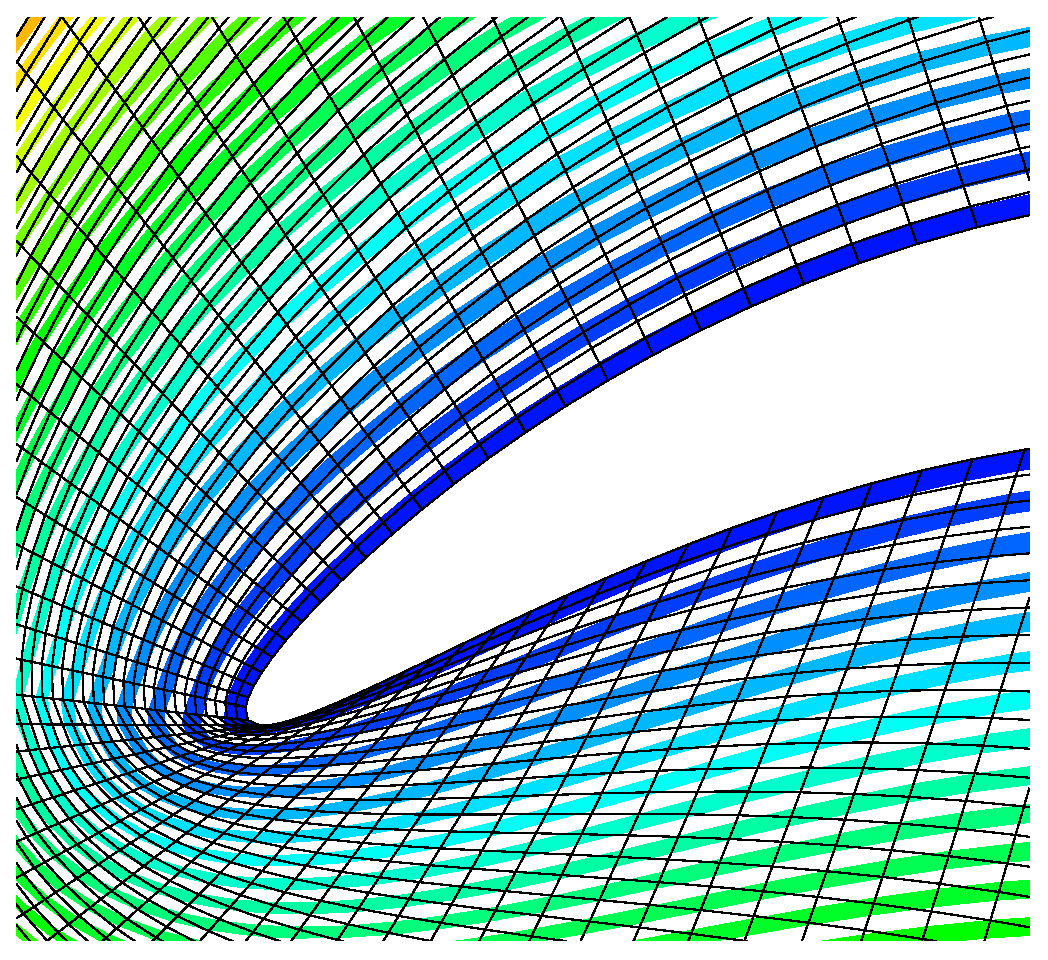
\includegraphics[width=0.5\textwidth]{Rysunki/NACA_8207_nosek_poisson}  
    	\quad      
    	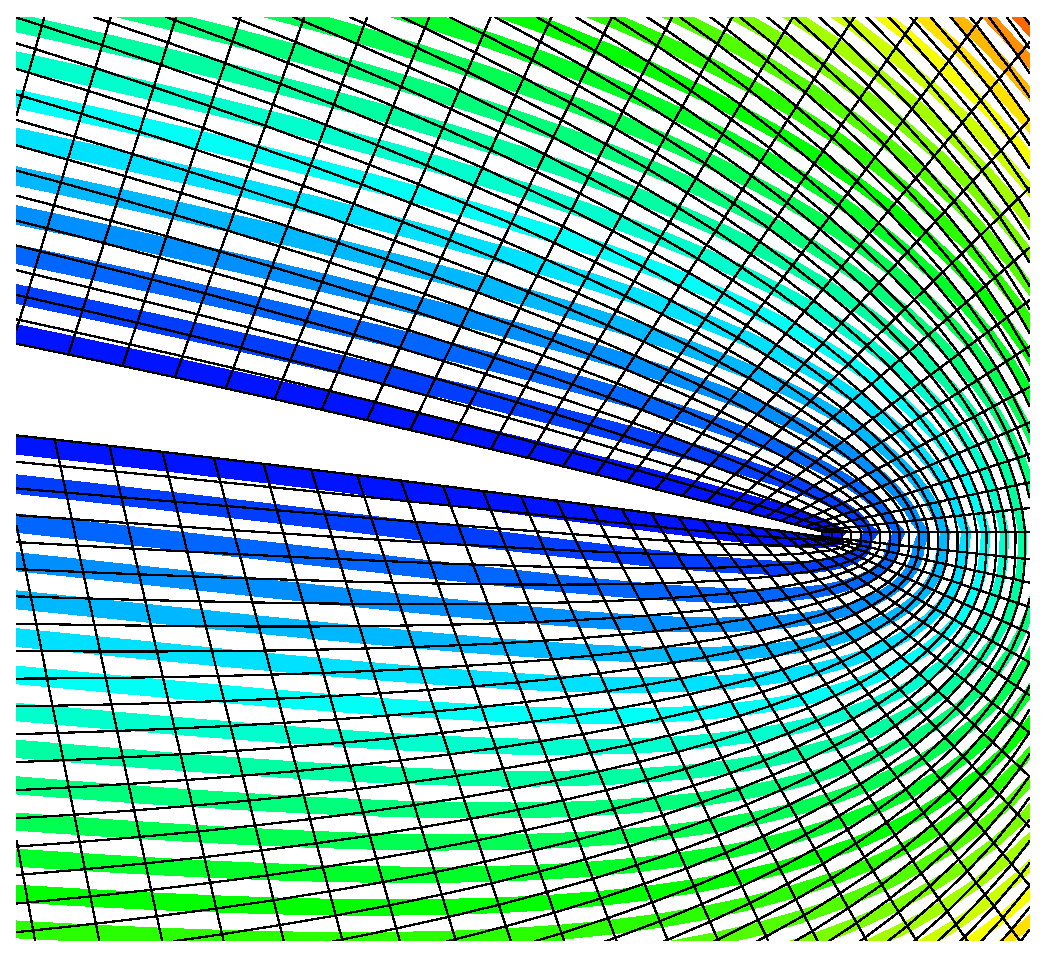
\includegraphics[width=0.5\textwidth]{Rysunki/NACA_8207_ostrze_poisson}		
		\subcaption{Metoda Poissona}
	\end{subfigure}
	\caption{Profil NACA 8207 (po lewej nosek profilu, po prawej ostrze)}
\end{figure}

\begin{figure}[b] 
	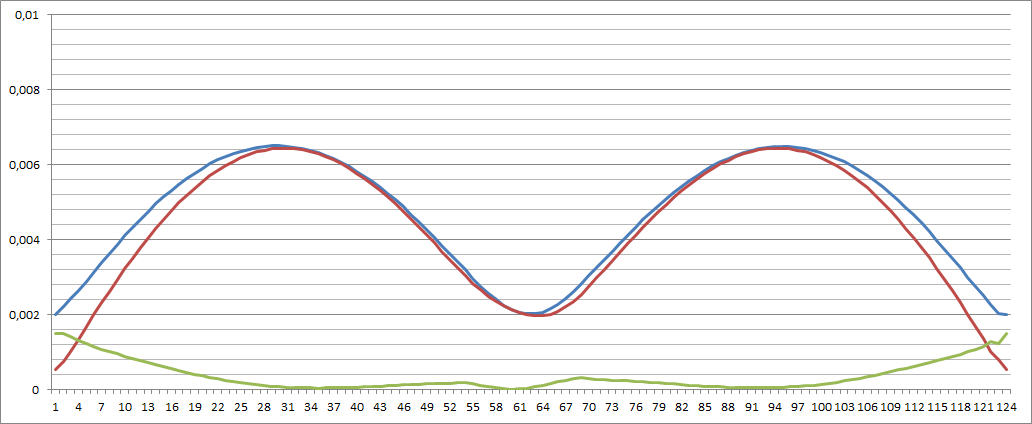
\includegraphics[trim = 30mm 0mm 0mm 0mm, width=1.1\linewidth]{Rysunki/NACA_0012_wykres_odleglosci.png}
	\caption{Wykres odległości dla pierwszego rzędu siatki dla metody \colorbox{red!30}{Poissona} i \colorbox{blue!30}{siłowej} (NACA 0012). Kolorem zielonym oznaczono \colorbox{green!30}{błąd bezwzględny}.}
	\label{fig:graph_NACA_0012}
\end{figure}

\begin{figure}[b] 
	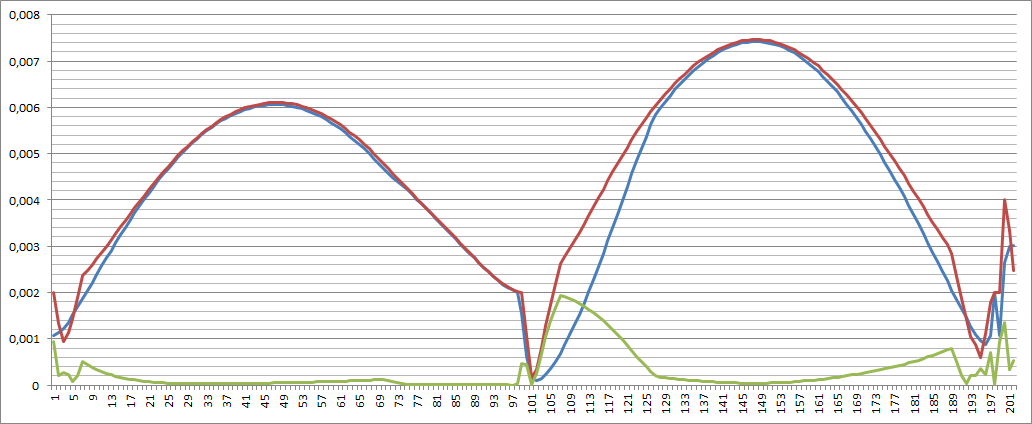
\includegraphics[trim = 30mm 0mm 0mm 0mm, width=1.1\linewidth]{Rysunki/NACA_8207_wykres_odleglosci.png}
	\caption{Wykres odległości dla pierwszego rzędu siatki dla metody \colorbox{blue!30}{Poissona} i \colorbox{red!30}{siłowej} (NACA 8207). Kolorem zielonym oznaczono \colorbox{green!30}{błąd bezwzględny}.}
	\label{fig:graph_NACA_8207}
\end{figure}
	\chapter{Wnioski}

\indent\indent Z wykresu (\ref{fig:graph_NACA_0012}) wynika, że odległość od brzegu wyznaczona metodą Poissona nie odbiega znacznie od dokładnej wartości obliczonej metodą siłową. Błąd w rejonie ostrza profilu można powiązać ze słabą jakością utworzonej tam siatki. Jest to również widoczne w rejonie noska i ostrza dla profilu o wygiętej szkieletowej \textsf{NACA 8207} (wykres \ref{fig:graph_NACA_8207}).

\begin{table}[h]\footnotesize
  \caption{Porównanie czasów wykonania metody siłowej i Poissona dla profili użytych w projekcie}
  \label{tab:comparision}
  \centering
\begin{tabular}{|c|c|c|}
\hline 
\rowcolor{light-gray} Metoda & NACA 0012 & NACA 8207 \\ 
\hline 
Siłowa  & 0.8 s & 2.1 s \\ 
\hline 
Równanie Poissona & 24 s & 30 s \\ 
\hline 
Ilość iteracji & 208 & 168 \\
\hline
Dokładność rozwiązania iteracyjnego & 0,09 & 0,07 \\
\hline\hline
\rowcolor{light-gray} Równanie Poissona & Czas & Iteracje\\
		\hline
		1) zerowy wektor początkowy & 24 s & 208 \\ 
		\hline
		2) dobrany wektor początkowy & 2.7 s & 14 \\
		\hline
\end{tabular} 
\end{table}

\indent Głównym mankamentem rozwiązania otrzymanego metodą Poissona jest czas wykonywania obliczeń, o rząd wielkości większy od rozwiązania siłowego (tab. \ref{tab:comparision}). Remedium jest spostrzeżenie, iż interesującym nas obszarem dokładnego rozwiązania jest bliskie sąsiedztwo brzegu profilu. Jeżeli udałoby się rozwiązać układ macierzowy w mniejszej liczbie iteracji, nie pogarszając przy tym wyników blisko brzegu, to zaoszczędzilibyśmy znaczną ilość czasu obliczeniowego. Taka możliwość istnieje, jeżeli zdefiniujemy wektor początkowy dla algorytmu iteracyjnego, o wartościach "z grubsza" odpowiadających rozkładowi rozwiązania w przestrzeni fizycznej\footnote{W programie zostało to zaimplementowane jako zainicjalizowanie zmiennej $\phi_i$ wartością \mbox{$i\cdot mod(n)\cdot \Delta$}}. Czas obliczeń  zbliża się wtedy do czasu wykonania metody siłowej (tab. \ref{tab:comparision}), a rozwiązanie w interesującym nas obszarze pozostaje poprawne (wykres \ref{fig:graph_NACA_0012_guess}).

\begin{figure}[h] 
	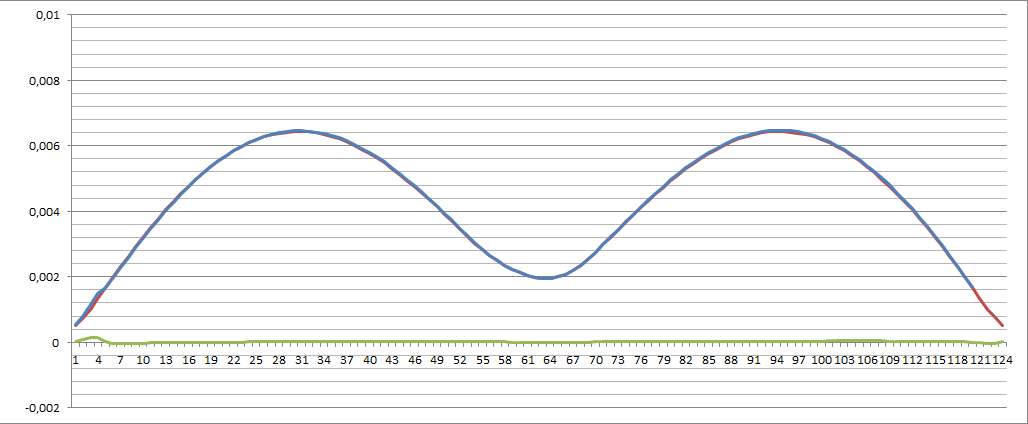
\includegraphics[trim = 30mm 0mm 0mm 0mm, width=1.1\linewidth]{Rysunki/NACA_0012_wykres_odleglosci_guess.png}
	\caption{Wykres odległości dla pierwszego rzędu siatki dla metody Poissona z \colorbox{red!30}{dobranym} wektorem początkowym i \colorbox{blue!30}{zerowym} (NACA 0012). Kolorem zielonym oznaczono \colorbox{green!30}{błąd bezwzględny}.}
	\label{fig:graph_NACA_0012_guess}
\end{figure}

\begin{figure}[H]	
    \centering
    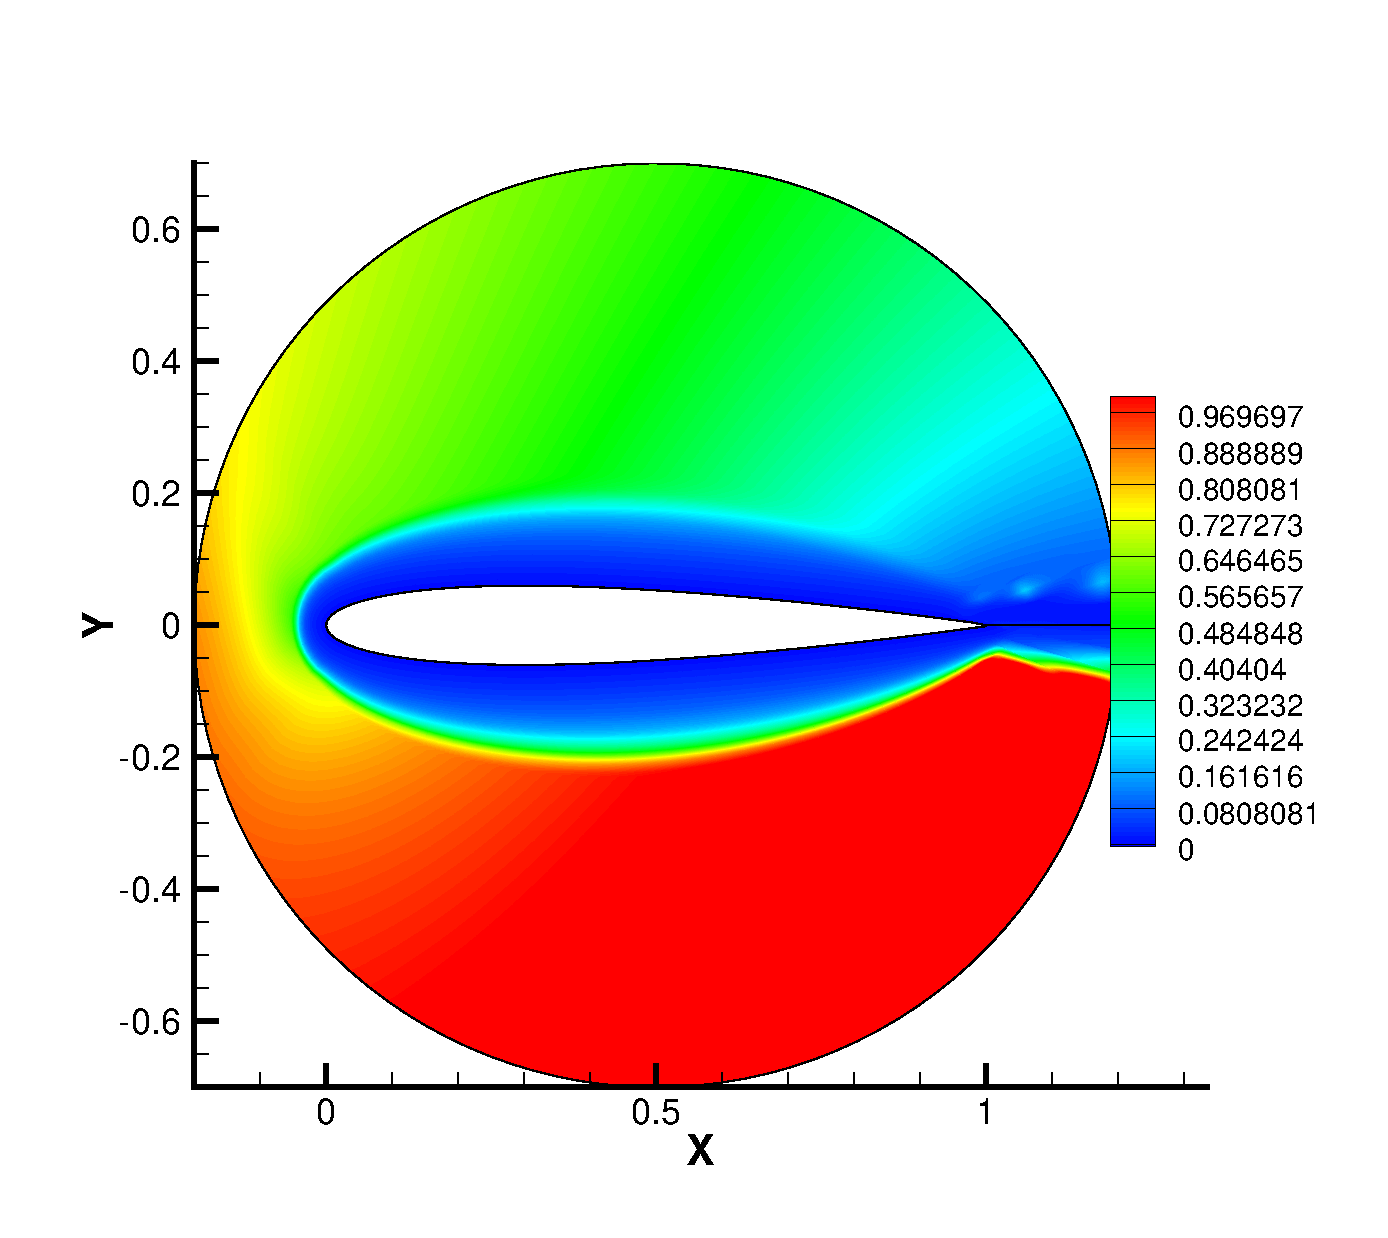
\includegraphics[trim = 22mm 10mm 10mm 20mm, width=0.9\linewidth]{Rysunki/NACA_0012_profil_poisson_guess.eps}    
	\caption{Rozwiązanie metodą Poissona otrzymane przy wykorzystaniu wektora początkowego}
\end{figure}

\section{Propozycje dalszego rozwoju}

\begin{enumerate}
	\item Jak wspomniano wcześniej, wybór iteracyjnej metody rozwiązania \mbox{\textsf{BiCSTAB}} związany był z dostępnością jej implementacji w bibliotece \textsf{Eigen}. Istnieją jednak dedykowane metody rozwiązania równania Poissona, które mogą przyspieszyć czas wykonywania programu. Jedną z nich jest \textsf{Fast Poisson Solver}, szerzej opisany w książce \textsf{Saada}\footcite{Saad, s. 58}.
	\item W oparciu o istniejącą architekturę programu należałoby dodać moduł rozwiązujący zagadnienie wykorzystując równanie Eikonału. Jest to równanie różniczkowe cząstkowe typu hiperbolicznego, dodatkowo nieliniowe. Implementacja będzie wymagać odmiennego modelu matematycznego oraz sposobu rozwiązania.
	\item Zamiast generować siatkę w programie, można ją otrzymać korzystając z pomocy zewnętrznego oprogramowania do preprocesingu (np. \mbox{\textsf{Gambit}})
\end{enumerate}	
	\renewcommand\bibname{Bibliografia}	%Zmiana nazwy z angielskiej na polską
\begin{thebibliography}{4}

\bibitem{Anderson}
	Anderson J.D.,
	\textsf{Computational Fluid Dynamics. The basics with applications},
	McGraw-Hill,
	1995.
	
\bibitem{Blazek}
	Blazek J.,
	\textsf{Computational Fluid Dynamics: Principles and Applications},
	Elsevier,
	2001.
	
\bibitem{Saad}
	Saad Y.
	\textsf{Iterative methods for sparse linear systems. Second edition.}
	SIAM,
	2003.
	
\bibitem{Sethain}
	Sethain J.A.
	\textsf{Level set methods and fast marching methods}.
	Cambridge University Press,
	1999.

\bibitem{Tucker}
	Tucker P.G.,
  	\textsf{Hybrid Hamilton-Jacobi-Poisson wall distance function model}.
  	Computers $\&$ Fluids 44,
  	(130-142),
  	2011.
  	
\end{thebibliography}


	
	\appendix							%Dodatki
	\chapter{Opis interfejsu programu}

\indent\indent Niniejszy dodatek opisuje sposób korzystania ze stworzonego w ramach niniejszego projektu programu \textsf{wallDistanceSolver.exe}, oraz jego interfejsu, do własnego użytku.

\section{Dane wejściowe}

\indent\indent Danymi wejściowymi do programu są współrzędne profilu zapisane w dwóch kolumnach, kolejno dla kierunku x oraz y, z użyciem kropki jako separatora dziesiętnego (kod źródłowy \ref{list:dane_wejściowe}). Domyślna nazwa pliku to \texttt{\mbox{NACA\_0012.dat}}

\begin{lstlisting}[label=list:dane_wejściowe,caption=Format zapisu danych wejściowych]
	0.964244   0.006169
	0.947231   0.008434
	........   ........
	........   ........	
\end{lstlisting}

\noindent\newline Sugeruje się nie pozostawiać pustych wierszy, złamanych znakiem nowej linii (enterem) na końcu kolumn, aby uniknąć możliwego wczytania nic nie znaczących znaków. Należy również zwrócić uwagę, aby wartości w wierszach nie powtarzały się, bowiem spowoduje to utworzenie kilku węzłów w tym samym punkcie, co przełoży się na rozwiązanie błędnie wygenerowanego układu równań \ref{eq:poisson_macierz}.   

\section{Dane wyjściowe}

\indent\indent Danymi wyjściowymi z programu są współrzędne $(x,y)$ węzłów siatki oraz wartość odległości od brzegu $d$, zapisane w trzech kolumnach w kolejności jak powyżej, z użyciem kropki jako separatora dziesiętnego (kod źródłowy \ref{list:dane_wyjściowe}). Dodatkowo program umożliwia wstawienie nagłówka niezbędnego do wczytania danych do oprogramowania \texttt{Tecplot 360}\footnote{\url{ftp://ftp.tecplot.com/pub/doc/tecplot/360/dataformat.pdf}, s. 134}

\begin{lstlisting}[label=list:dane_wyjściowe,caption=Format zapisu danych wyjściowych]
\end{lstlisting}\begin{center}
\underline{Zwykłe formatowanie}
\end{center}
\begin{lstlisting}  
              1              0              0
       0.979641       0.004079              0
       0.964244       0.006169              0 
       ........       ........       ........
       0.850307       0.032659       0.012574
       0.831428       0.035881       0.013543
	   ........       ........	     ........	
\end{lstlisting}
\begin{center}
\underline{Format danych programu Tecplot 360}
\end{center}
\begin{lstlisting}  
	VARIABLES = "X", "Y", "U",
	ZONE I=124, J=41, DATAPACKING=POINT

              1              0              0
       0.979641       0.004079              0
       0.964244       0.006169              0 
       ........       ........       ........
       0.850307       0.032659       0.012574
       0.831428       0.035881       0.013543
	   ........       ........	     ........
\end{lstlisting}


\section{Przykładowy program}

\indent\indent W pierwszym kroku definiowane są zmienne pomocnicze, określające promień siatki \textsf{circleRadius}, liczbę rzędów \textsf{gridDensity} oraz położenie jej środka \textsf{S} (korzystając z  klasy pomocniczej \textsf{cPoint}).

Następnie następuje inicjalizacja obiektu solvera \textsf{CASE}, oraz wczytanie z pliku współrzędnych punktów profilu metodą \textsf{addProfile()}. Na podstawie tych danych tworzona jest siatka o wcześniej zdefiniowanych parametrach (metoda \textsf{generateGrid()}). Rozwiązanie zagadnienia odbywa się przy użyciu metody \textsf{solve(POISSON)}\footnote{Dla celów porównawczych można skorzystać z metody siłowej. W tym celu należy zmienić typ wyliczeniowy z \textsf{POISSON} na \textsf{BRUTE\_FORCE}.}

W ostatnim kroku otrzymane rozwiązanie jest zapisywane metodą \\ \mbox{\textsf{saveSolution()}}. Treść komunikatów programu przedstawiono w kodzie źródłowym (\ref{list:konsola}).

\begin{lstlisting}[label=list:program,caption=Przykładowy program rozwiązujący zagadnienie]
	#include <iostream>
	#include "cSolver.h"

	int main(int argc, char * argv[]){
		//Grid parametres
		cPoint	S				= cPoint(0.5, 0.0);	
		double	circleRadius	= 1;
		int		gridDensity		= 40;

		cSolver CASE;

		//Read profile from a file
		CASE.addProfile("../../data/NACA_0012.dat");

		//Generate grid based on profile
		CASE.generateGrid(S, circleRadius, gridDensity);

		//Solve problem
		std::cout << CASE.solve(POISSON) << std::endl;
	
		//Save solution to a file
		CASE.saveSolution(DISTANCE);	
	
		return 0;
	}
\end{lstlisting}


\begin{lstlisting}[label=list:konsola,caption=Widok konsoli programu]
	Generating grid
	Grid generated!
	Solving Poisson...
		#iterations: 81	estimated error: 1.83435e-06
	Solution solved!
	6.908
	Saving solution...
	Solution saved!
\end{lstlisting}
					%Opis interfejsu programu
	\chapter{Zawartość płyty CD}

\noindent Pliki źródłowe programu (folder \textsf{Source files})
\begin{itemize}
	\item[o] \textsf{main.cpp} 
	\item[o] \textsf{cPoint.cpp} 
	\item[o] \textsf{cSolution.cpp} 
	\item[o] \textsf{cSolver.cpp} 
	\item[o] \textsf{cGrid.cpp} 
\end{itemize}

\noindent Pliki nagłówkowe (folder \textsf{Source files})
\begin{itemize}
	\item[o] \textsf{cPoint.h} 
	\item[o] \textsf{cSolution.h} 
	\item[o] \textsf{cSolver.h} 
	\item[o] \textsf{cGrid.h} 
\end{itemize}

\noindent Przykładowy program (folder \textsf{Source files})
\begin{itemize}
	\item[o] \textsf{wallDistanceSolver.exe}
\end{itemize}

\noindent Pliki wejściowe (folder \textsf{Data})
\begin{itemize}
	\item[o] \textsf{NACA\_0012.dat} - współrzędne x,y profilu NACA~0012
	\item[o] \textsf{NACA\_8207.dat} - współrzędne x,y profilu NACA~8207
\end{itemize}

\noindent Dokumentacja
\begin{itemize}
	\item[o] \textsf{Dokumentacja.pdf} - wersja cyfrowa niniejszego opracowania
\end{itemize}
					%Zawartość płyty CD
\end{document}